\documentclass[12pt,a4paper]{article}

% ==============================================================================
% ПРЕАМБУЛА: Учебно-методическое пособие по дисциплине
% «Физические основы нанотехнологий» (ГУАП, Кафедра №3)
% ==============================================================================

\usepackage[T2A]{fontenc}
\usepackage[utf8]{inputenc}
\usepackage[russian]{babel}

% Геометрия страницы по университетскому стандарту
\usepackage[a4paper, top=20mm, bottom=20mm, left=25mm, right=15mm, headheight=15pt]{geometry}

% Нумерация в стиле «Глава 2» (2.X)
\renewcommand{\thesection}{2.\arabic{section}}
\renewcommand{\thesubsection}{2.\arabic{section}.\arabic{subsection}}
\renewcommand{\thesubsubsection}{2.\arabic{section}.\arabic{subsection}.\arabic{subsubsection}}
\renewcommand{\theequation}{2.\arabic{equation}}
\renewcommand{\thefigure}{2.\arabic{figure}}
\renewcommand{\thetable}{2.\arabic{table}}

% Типографика и микротипографика
\usepackage{microtype}
\usepackage{indentfirst}
\setlength{\parindent}{1.25cm}
\setlength{\parskip}{2pt plus 1pt minus 1pt}
\linespread{1.15}

% Математические пакеты
\usepackage{amsmath,amssymb,mathtools,bm}

% Таблицы
\usepackage{booktabs}
\usepackage{tabularx}
\usepackage{array}
\usepackage{multirow}

% Графика и подрисунки
\usepackage{graphicx}
\usepackage{caption}
\usepackage{subcaption}
\captionsetup{font=small, labelfont=bf, labelsep=period, justification=centering}
\captionsetup[sub]{font=small, labelfont=bf, labelsep=space}

% Цветовая палитра ГУАП
\usepackage{xcolor}
\definecolor{guapblue}{RGB}{0, 44, 95}       % Фирменный темно-синий ГУАП
\definecolor{guapaccent}{RGB}{0, 102, 204}   % Небесно-голубой акцент
\definecolor{darkslate}{RGB}{36, 40, 52}     % Основной текст
\definecolor{examplegreen}{RGB}{24, 115, 60} % Зеленый для примеров задач
\definecolor{amberdark}{RGB}{185, 110, 0}    % Янтарный для замечаний
\definecolor{bordergray}{RGB}{210, 215, 225}

% Выделенные блоки tcolorbox
\usepackage{tcolorbox}
\tcbuselibrary{skins,breakable}

% 1. Определение
\newtcolorbox{defbox}[1]{
    enhanced,
    breakable,
    colback=guapblue!4!white,
    colframe=guapblue,
    coltitle=white,
    fonttitle=\bfseries\sffamily,
    title=Определение: #1,
    arc=2mm,
    boxrule=1pt,
    top=3mm, bottom=3mm, left=3mm, right=3mm
}

% 2. Закон / Правило
\newtcolorbox{lawbox}[1]{
    enhanced,
    breakable,
    colback=guapaccent!5!white,
    colframe=guapaccent!85!black,
    coltitle=white,
    fonttitle=\bfseries\sffamily,
    title=Закон / Правило: #1,
    arc=2mm,
    boxrule=1pt,
    top=3mm, bottom=3mm, left=3mm, right=3mm
}

% 3. Пример решения задачи
\newtcolorbox{exbox}[1]{
    enhanced,
    breakable,
    colback=examplegreen!4!white,
    colframe=examplegreen,
    coltitle=white,
    fonttitle=\bfseries\sffamily,
    title=Пример решения задачи: #1,
    arc=2mm,
    boxrule=1pt,
    top=3mm, bottom=3mm, left=3mm, right=3mm
}

% 4. Методическое замечание / Важное указание
\newtcolorbox{notebox}[1]{
    enhanced,
    breakable,
    colback=amberdark!5!white,
    colframe=amberdark,
    coltitle=white,
    fonttitle=\bfseries\sffamily,
    title=Методическое замечание: #1,
    arc=2mm,
    boxrule=1pt,
    top=3mm, bottom=3mm, left=3mm, right=3mm
}

% 5. Контрольные вопросы и задания
\newtcolorbox{questbox}[1]{
    enhanced,
    breakable,
    colback=guapblue!3!white,
    colframe=guapblue!70!black,
    coltitle=white,
    fonttitle=\bfseries\sffamily,
    title=Задание для самопроверки: #1,
    arc=2mm,
    boxrule=0.8pt,
    top=3mm, bottom=3mm, left=3mm, right=3mm
}

% Оформление колонтитулов
\usepackage{fancyhdr}
\pagestyle{fancy}
\fancyhf{}
\fancyhead[L]{\small\sffamily\textcolor{guapblue}{Физические основы нанотехнологий}}
\fancyhead[R]{\small\sffamily\textcolor{guapblue}{Глава 2. Термодинамика наноструктур}}
\fancyfoot[C]{\sffamily\thepage}
\renewcommand{\headrulewidth}{0.5pt}
\renewcommand{\footrulewidth}{0pt}

% Ссылки и навигация
\usepackage[unicode, colorlinks=true, linkcolor=guapblue, citecolor=examplegreen, urlcolor=guapaccent]{hyperref}

% Заголовки разделов
\usepackage{titlesec}
\titleformat{\section}
  {\normalfont\Large\bfseries\sffamily\color{guapblue}}{\thesection}{1em}{}
\titleformat{\subsection}
  {\normalfont\large\bfseries\sffamily\color{guapblue!85!black}}{\thesubsection}{1em}{}
\titleformat{\subsubsection}
  {\normalfont\normalsize\bfseries\sffamily\color{guapblue!70!black}}{\thesubsubsection}{1em}{}

% Путь к рисункам
\graphicspath{{figures/}}


\begin{document}

\begin{center}
{\Large\bfseries\sffamily\color{guapblue} ГЛАВА 2}\\[0.3em]
{\LARGE\bfseries\sffamily\color{guapblue} Термодинамические основы наноструктур и фазовые равновесия}
\end{center}
\vspace{1em}

% ==============================================================================
% 2.1. Введение и базовые понятия
% ==============================================================================
\section{Введение и базовые понятия феноменологической термодинамики}
\label{sec:intro}

Термодинамика представляет собой макроскопическую науку о закономерностях превращения различных форм энергии и направлениях самопроизвольного протекания физико-химических процессов. В отличие от статистической физики и квантовой механики, оперирующих координатами, импульсами и волновыми функциями отдельных частиц, феноменологическая термодинамика описывает систему ограниченным набором макроскопических параметров состояния: температурой $T$, давлением $P$, объемом $V$ и количествами компонентов $n_1, n_2, \dots, n_k$.

\begin{defbox}{Термодинамическая система и состояние}
\textbf{Термодинамической системой} называется выделенная реальными или мысленными границами совокупность материальных тел, взаимодействующая с окружающей средой путем обмена энергией и/или веществом.

Совокупность независимых макроскопических параметров полностью определяет \textbf{термодинамическое состояние} системы. Функции параметров состояния, значения которых однозначно фиксируются состоянием системы и не зависят от предыстории процесса, называются \textbf{функциями состояния} ($U, S, H, F, G$).
\end{defbox}

\subsection{Внутренняя энергия: микроскопическая природа}
Центральным понятием термодинамики является \textbf{внутренняя энергия} $U$. Необходимо строго разграничивать механическую энергию тела как единого целого (например, кинетическую энергию летящего объекта $E_k = \frac{1}{2}m v^2$ или гравитационную потенциальную энергию $E_p = mgh$) и его внутреннюю энергию. Термодинамику интересует исключительно энергия микроскопического хаотического движения и взаимодействия структурных единиц вещества.

Внутренняя энергия $U$ складывается из двух основных вкладов:
\begin{equation}
U = E_{\mathrm{kin}}^{\mathrm{micro}} + E_{\mathrm{pot}}^{\mathrm{micro}},
\label{eq:internal_energy}
\end{equation}
где $E_{\mathrm{kin}}^{\mathrm{micro}}$ --- суммарная кинетическая энергия хаотического поступательного, вращательного и колебательного движения атомов и молекул (макроскопически воспринимаемая как абсолютная температура $T$); $E_{\mathrm{pot}}^{\mathrm{micro}}$ --- потенциальная энергия межмолекулярного и межатомного взаимодействия (силы Ван-дер-Ваальса, ковалентные, ионные и металлические связи), определяющая агрегатное состояние вещества.

\subsection{Теплота и работа как формы передачи энергии}
Распространенной методической ошибкой является утверждение о том, что тело «содержит в себе теплоту или работу». Тело содержит исключительно внутреннюю энергию $U$. \textbf{Теплота} $Q$ и \textbf{работа} $A$ представляют собой не формы хранения, а \textbf{два принципиально различных способа передачи энергии} через границу раздела системы:
\begin{itemize}
    \item \textbf{Работа ($A$ или $W$):} макроскопически упорядоченная форма передачи энергии, сопряженная с перемещением границ системы под действием обобщенных сил (например, механическая работа сжатия газа поршнем $\delta A = P\,dV$ или работа образования новой поверхности $\delta A = -\sigma\,dA$). При этом молекулы приграничного слоя получают согласованное направленное движение.
    \item \textbf{Теплота ($Q$):} микроскопически хаотическая, неупорядоченная форма передачи энергии, реализуемая через стохастические соударения частиц на границе раздела контактирующих тел с различной температурой.
\end{itemize}

\begin{lawbox}{Первое начало термодинамики}
В соответствии с законом сохранения энергии, изменение внутренней энергии замкнутой системы равно разности полученного системой тепла и совершенной ею работы над внешними телами:
\begin{equation}
dU = \delta Q - \delta A.
\label{eq:first_law}
\end{equation}
Знак дифференциала $d$ подчеркивает, что внутренняя энергия $U$ является строгим полным дифференциалом (функцией состояния), тогда как элементарные количества тепла $\delta Q$ и работы $\delta A$ полными дифференциалами не являются и зависят от пути процесса.
\end{lawbox}

\subsection{Второе начало термодинамики и энтропия}
Первое начало запрещает возникновение энергии из ничего (вечный двигатель I рода), но не накладывает никаких ограничений на направление передачи энергии. Второе начало термодинамики формулирует вектор самопроизвольных процессов: теплота самопроизвольно переходит только от более нагретого тела к менее нагретому.

Количественной мерой необратимости и неупорядоченности системы служит \textbf{энтропия} $S$, определяемая для квазистатических обратимых процессов соотношением Клаузиуса:
\begin{equation}
dS = \frac{\delta Q_{\mathrm{rev}}}{T}.
\label{eq:entropy_def}
\end{equation}
В изолированной макросистеме ($\delta Q = 0$) энтропия не может убывать: $dS \ge 0$, достигая абсолютного максимума в состоянии термодинамического равновесия.

% ==============================================================================
% 2.2. Термодинамические потенциалы
% ==============================================================================
\section{Термодинамические потенциалы и условия фазового равновесия}
\label{sec:potentials}

Для систем, находящихся в контакте с окружающей средой при заданных внешних параметрах, использование энтропии $S(U, V)$ неудобно, поскольку естественными переменными экспериментатора в лаборатории являются температура $T$ и давление $P$. Для этого Дж.~В.~Гиббс разработал математический аппарат \textbf{характеристических функций} (термодинамических потенциалов), получаемых преобразованием Лежандра из внутренней энергии:

\begin{enumerate}
    \item \textbf{Энтальпия ($H$):} $H = U + PV$, естественные переменные $(S, P)$.
    \begin{equation}
    dH = T\,dS + V\,dP + \sum_{i=1}^k \mu_i\,dn_i.
    \end{equation}
    \item \textbf{Свободная энергия Гельмгольца ($F$):} $F = U - TS$, естественные переменные $(T, V)$.
    \begin{equation}
    dF = -S\,dT - P\,dV + \sum_{i=1}^k \mu_i\,dn_i.
    \end{equation}
    \item \textbf{Свободная энергия Гиббса ($G$):} $G = H - TS = U + PV - TS$, естественные переменные $(T, P)$.
    \begin{equation}
    dG = -S\,dT + V\,dP + \sum_{i=1}^k \mu_i\,dn_i.
    \label{eq:dg_fundamental}
    \end{equation}
\end{enumerate}

\subsection{Энергия Гиббса и критерий самопроизвольности}
В условиях подавляющего большинства лабораторных и промышленных процессов синтеза наноматериалов реактор находится при постоянной температуре ($T = \mathrm{const}$) и атмосферном давлении ($P = \mathrm{const}$). При этих условиях фундаментальное уравнение~(\ref{eq:dg_fundamental}) сводится к:
\begin{equation}
(dG)_{T,P} \le 0.
\label{eq:gibbs_criterion}
\end{equation}
Свободная энергия Гиббса представляет собой баланс между стремлением системы к минимуму потенциальной энергии межатомного взаимодействия (энтальпийный фактор $H$) и максимуму молекулярного хаоса (энтропийный фактор $-TS$). \textbf{Любой самопроизвольный процесс в изобарно-изотермической системе протекает исключительно в направлении уменьшения энергии Гиббса ($\Delta G < 0$)}, а состояние устойчивого термодинамического равновесия соответствует минимуму свободной энергии ($G = \mathrm{min}, dG = 0$).

\subsection{Химический потенциал как мера реакционной способности}
Для систем с переменным числом частиц ключевым интенсивным параметром выступает \textbf{химический потенциал} $\mu_i$, введенный Гиббсом как частная производная энергии Гиббса по количеству $i$-го компонента:

\begin{defbox}{Химический потенциал}
\textbf{Химическим потенциалом} $\mu_i$ $i$-го компонента в фазе называется приращение свободной энергии Гиббса системы при добавлении в данную фазу одного моля (или одной частицы) этого компонента при фиксированных температуре, давлении и неизменных количествах всех остальных компонентов:
\begin{equation}
\mu_i = \left( \frac{\partial G}{\partial n_i} \right)_{T, P, n_{j \ne i}}.
\label{eq:chem_pot_def}
\end{equation}
\end{defbox}

\begin{notebox}{Физическая аналогия химического потенциала}
Химический потенциал $\mu$ играет в термодинамике диффузии и фазовых превращений точно такую же роль, как температура $T$ в теплообмене или электрический потенциал $\varphi$ в электродинамике:
\begin{itemize}
    \item Теплота перетекает от большего $T$ к меньшему $T$.
    \item Электрический заряд течет от большего потенциала $\varphi$ к меньшему $\varphi$.
    \item \textbf{Вещество самопроизвольно перетекает из фазы с большим химическим потенциалом в фазу с меньшим химическим потенциалом.}
\end{itemize}
Химический потенциал можно понимать как «энергетическую цену» размещения дополнительной частицы в данной кристаллической или жидкой структуре. Вещество переходит туда, где эта «цена» минимальна.
\end{notebox}

\subsection{Фундаментальное условие фазового равновесия}
Пусть система состоит из двух фаз $\alpha$ и $\beta$, между которыми происходит обмен частицами $i$-го компонента при $T, P = \mathrm{const}$. Полное изменение энергии Гиббса составляет:
\begin{equation}
dG = \mu_i^{(\alpha)}\,dn_i^{(\alpha)} + \mu_i^{(\beta)}\,dn_i^{(\beta)}.
\end{equation}
Поскольку общее количество вещества сохраняется ($dn_i^{(\alpha)} + dn_i^{(\beta)} = 0$, то есть $dn_i^{(\beta)} = -dn_i^{(\alpha)}$):
\begin{equation}
dG = \left( \mu_i^{(\alpha)} - \mu_i^{(\beta)} \right) dn_i^{(\alpha)}.
\end{equation}
Если $\mu_i^{(\alpha)} > \mu_i^{(\beta)}$, то для обеспечения $dG < 0$ требуется $dn_i^{(\alpha)} < 0$ --- вещество самопроизвольно покидает фазу $\alpha$ и переходит в фазу $\beta$ (например, лед тает в воду при $+1^\circ\mathrm{C}$, поскольку химический потенциал льда выше химического потенциала воды). 

В состоянии равновесия $dG = 0$, откуда вытекает строгое условие:

\begin{lawbox}{Условие межфазного термодинамического равновесия}
Необходимым и достаточным условием равновесного сосуществования фаз в многофазной гетерогенной системе является равенство температур, давлений и химических потенциалов каждого из компонентов во всех сосуществующих фазах:
\begin{equation}
T^{(\alpha)} = T^{(\beta)} = \dots = T^{(\Phi)}, \qquad P^{(\alpha)} = P^{(\beta)} = \dots = P^{(\Phi)},
\end{equation}
\begin{equation}
\mu_i^{(\alpha)} = \mu_i^{(\beta)} = \dots = \mu_i^{(\Phi)} \qquad (i = 1, 2, \dots, k).
\label{eq:phase_equilibrium_condition}
\end{equation}
\end{lawbox}

% ==============================================================================
% 2.3. Правило фаз Гиббса
% ==============================================================================
\section{Правило фаз Гиббса}
\label{sec:phase_rule}

Правило фаз Гиббса связывает между собой число степеней свободы гетерогенной системы $f$ с числом ее компонентов $k$ и числом находящихся в равновесии фаз $\varphi$.

\begin{defbox}{Степень свободы термодинамической системы}
\textbf{Числом термодинамических степеней свободы} (вариантностью системы) $f$ называется количество независимых интенсивных параметров состояния (температура, давление, концентрации компонентов в фазах), которые можно произвольно изменять в некоторых пределах без изменения числа и природы равновесных фаз.
\end{defbox}

\subsection{Термодинамический вывод правила фаз}
Рассмотрим систему, содержащую $k$ независимых компонентов, распределенных между $\varphi$ сосуществующими фазами:
\begin{enumerate}
    \item \textbf{Подсчет числа переменных:}
    Термодинамическое состояние каждой фазы описывается температурой $T$, давлением $P$ и мольными долями компонентов $x_{1}, x_{2}, \dots, x_{k}$. Так как сумма мольных долей равна единице ($\sum_{i=1}^k x_i = 1$), состав каждой фазы независимым образом задается $(k - 1)$ переменными. Для $\varphi$ фаз получаем $\varphi(k - 1)$ концентрационных параметров. 
    С учетом общих для всех фаз $T$ и $P$, общее число интенсивных переменных системы равно:
    \begin{equation}
    N_{\mathrm{var}} = \varphi(k - 1) + 2.
    \end{equation}
    \item \textbf{Подсчет числа уравнений связи:}
    Условие фазового равновесия~(\ref{eq:phase_equilibrium_condition}) требует равенства химических потенциалов каждого компонента во всех фазах:
    \begin{equation}
    \mu_i^{(1)} = \mu_i^{(2)} = \dots = \mu_i^{(\varphi)} \qquad (i = 1, 2, \dots, k).
    \end{equation}
    Для каждого $i$-го компонента имеется цепочка из $(\varphi - 1)$ независимых равенств. Для всех $k$ компонентов общее число уравнений связи составляет:
    \begin{equation}
    N_{\mathrm{eq}} = k(\varphi - 1).
    \end{equation}
    \item \textbf{Нахождение вариантности $f$:}
    Число степеней свободы равно разности между числом переменных и числом уравнений связи:
    \begin{equation}
    f = N_{\mathrm{var}} - N_{\mathrm{eq}} = \varphi(k - 1) + 2 - k(\varphi - 1) = \varphi k - \varphi + 2 - k\varphi + k.
    \end{equation}
\end{enumerate}

Сокращая члены, получаем классическое уравнение Гиббса:
\begin{equation}
f = k - \varphi + 2.
\label{eq:gibbs_phase_rule}
\end{equation}

Если процесс проводится при постоянном внешнем давлении (например, изобарические условия в открытом тигле при $P = \mathrm{const} = 1\text{ атм}$), одна степень свободы исключается, и правило фаз принимает вид:
\begin{equation}
f = k - \varphi + 1.
\label{eq:gibbs_phase_rule_isobaric}
\end{equation}

\subsection{Анализ степеней свободы однокомпонентной системы ($k = 1$)}
На рис.~\ref{fig:degrees_of_freedom} проиллюстрировано применение правила фаз Гиббса на примере фазовой диаграммы $P\text{--}T$ воды ($k = 1$):
\begin{itemize}
    \item \textbf{Однофазная область ($\varphi = 1$, только пар или только жидкая вода):}
    \begin{equation*}
    f = 1 - 1 + 2 = 2 \quad (\text{бивариантная система}).
    \end{equation*}
    Можно независимо варьировать как температуру $T$, так и давление $P$ внутри области, не вызывая фазового превращения.
    \item \textbf{Линия фазового равновесия ($\varphi = 2$, лед + вода или вода + пар):}
    \begin{equation*}
    f = 1 - 2 + 2 = 1 \quad (\text{моновариантная система}).
    \end{equation*}
    Остается только одна свободная «ручка управления». Если исследователь задает температуру $T$, равновесное давление $P$ жестко фиксируется кривой равновесия (уравнение Клапейрона--Клаузиуса).
    \item \textbf{Тройная точка ($\varphi = 3$, лед + вода + пар сосуществуют одновременно):}
    \begin{equation*}
    f = 1 - 3 + 2 = 0 \quad (\text{нонвариантная точка}).
    \end{equation*}
    Свободных параметров нет. Тройная точка воды реализуется при строго единственной комбинации параметров: $T = 0.01^\circ\mathrm{C}$ ($273.16\text{ К}$), $P = 611.65\text{ Па}$. Любое изменение давления или температуры неминуемо приведет к исчезновению хотя бы одной из трех фаз.
\end{itemize}

\begin{figure}[htbp]
    \centering
    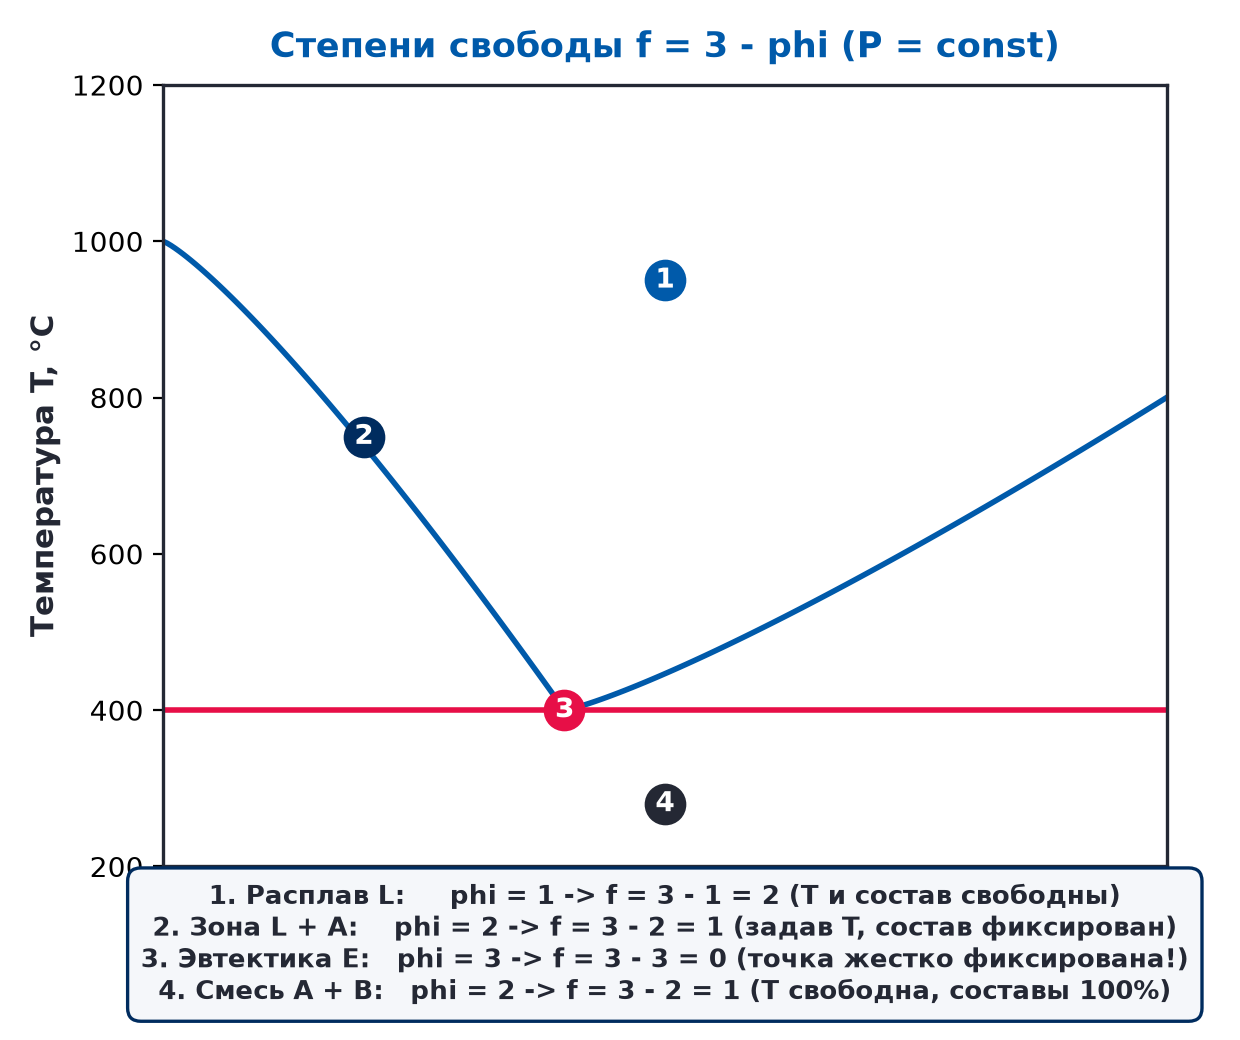
\includegraphics[width=0.88\textwidth]{fig_degrees_of_freedom.png}
    \caption{Степени свободы термодинамической системы и геометрический смысл правила фаз Гиббса $f = k - \varphi + 2$ на плоскости $P\text{--}T$ для однокомпонентной системы ($k = 1$): однофазные поля ($f = 2$), линии фазового перехода ($f = 1$) и тройная точка ($f = 0$).}
    \label{fig:degrees_of_freedom}
\end{figure}

% ==============================================================================
% 2.4. Бинарные фазовые диаграммы и термический анализ
% ==============================================================================
\section{Бинарные фазовые диаграммы и термический анализ}
\label{sec:binary_diagrams}

В физике наноструктур и полупроводниковом материаловедении определяющую роль играют двухкомпонентные (бинарные) системы ($k = 2$). Для бинарных сплавов диаграммы строятся в изобарических координатах «температура --- состав» ($T\text{--}C$) при фиксированном давлении $P = 1\text{ атм}$. Состав сплава обычно выражается в атомных процентах ($\text{ат. } \% $) или массовых процентах ($\text{мас. } \% $) второго компонента.

\subsection{Анатомия бинарной диаграммы}
Бинарная диаграмма состояния содержит ключевые топологические элементы:
\begin{itemize}
    \item \textbf{Линия ликвидуса (liquidus):} геометрическое место точек температур, выше которых сплав любого состава находится исключительно в гомогенном жидком состоянии ($L$). При охлаждении расплава линия ликвидуса соответствует началу кристаллизации.
    \item \textbf{Линия солидуса (solidus):} геометрическое место точек температур, ниже которых сплав полностью затвердевает и жидкая фаза отсутствует.
    \item \textbf{Двухфазная область ($L + S$):} область сосуществования жидкости и кристаллов. Согласно правилу фаз при $P = \mathrm{const}$:
    \begin{equation*}
    f = k - \varphi + 1 = 2 - 2 + 1 = 1.
    \end{equation*}
    Внутри двухфазной области температура однозначно фиксирует составы равновесных жидкой и твердой фаз.
    \item \textbf{Эвтектическая точка ($E$):} особая точка, в которой жидкий расплав кристаллизуется при минимальной для данной системы температуре $T_E$ с одновременным выделением смеси двух твердых фаз:
    \begin{equation}
    L_E \xrightarrow{T_E} \alpha + \beta.
    \label{eq:eutectic_reaction}
    \end{equation}
    В эвтектической точке сосуществуют три фазы ($\varphi = 3$: расплав $L$, чистый твердый $A$ и чистый твердый $B$). По правилу фаз:
    \begin{equation*}
    f = 2 - 3 + 1 = 0.
    \end{equation*}
    Эвтектическая кристаллизация нонвариантна и протекает при строго постоянной температуре $T_E$ до полного исчерпания жидкой фазы.
\end{itemize}

\subsection{Метод термического анализа и синтез диаграммы}
Исторически и технологически фазовые диаграммы строятся экспериментальным методом \textbf{термического анализа}. Образцы расплавов чистых компонентов и смесей с различной концентрацией $C_1, C_2, \dots$ медленно охлаждают в печи с непрерывной регистрацией термопарой зависимости температуры от времени $T(t)$ --- кривых охлаждения.

\begin{figure}[htbp]
    \centering
    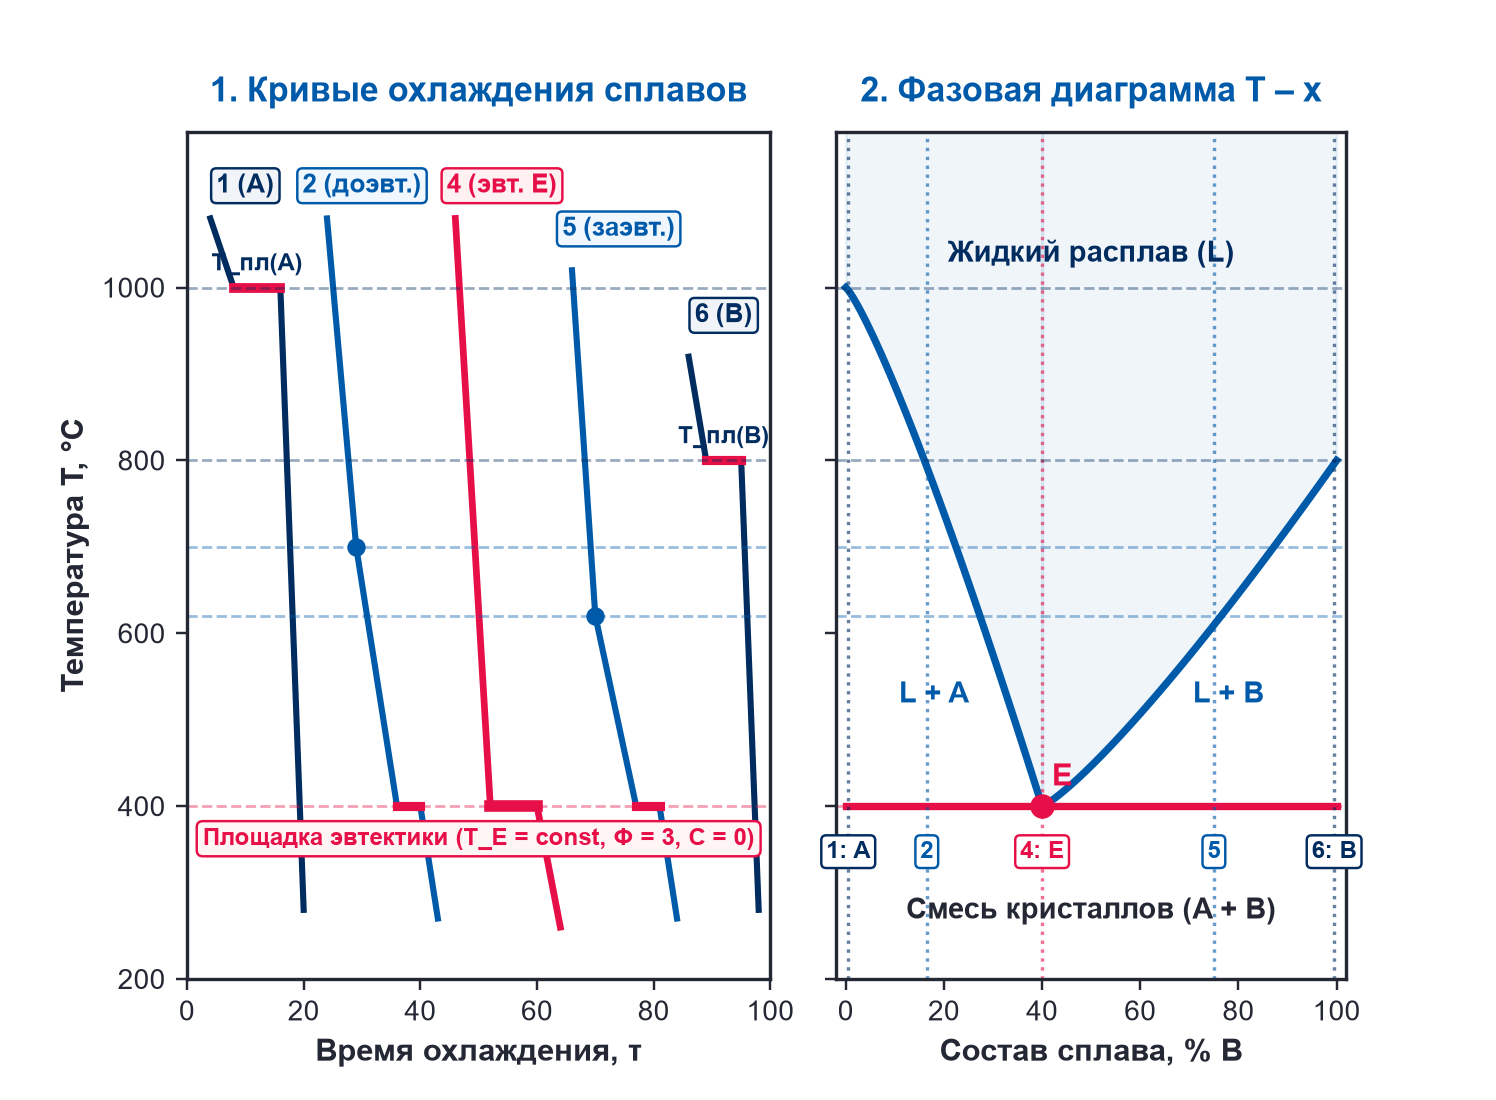
\includegraphics[width=0.92\textwidth]{fig_thermal_analysis.png}
    \caption{Синтез фазовой диаграммы бинарной системы методом термического анализа: (а) кривые охлаждения для чистого золота (1), доэвтектического сплава 10\% Si (2), эвтектического состава 18.6\% Si (3) и кремния (4); (б) перенос температур фазовых переходов на координатную плоскость $T\text{--}C$; (в) итоговая фазовая диаграмма эвтектического типа $\mathrm{Au\text{--}Si}$.}
    \label{fig:thermal_analysis}
\end{figure}

На рис.~\ref{fig:thermal_analysis} продемонстрирована последовательность синтеза диаграммы состояния $\mathrm{Au\text{--}Si}$:
\begin{enumerate}
    \item \textbf{Кривая 1 (Чистое золото, $k = 1$):} охлаждение жидкого расплава идет непрерывно до точки плавления $T_m(\mathrm{Au}) = 1064^\circ\mathrm{C}$. В процессе кристаллизации сосуществуют две фазы ($\varphi = 2$, расплав + кристаллы), поэтому $f = 1 - 2 + 1 = 0$. На кривой охлаждения формируется горизонтальная \textbf{термическая остановка (температурная площадка)}: выделяющаяся скрытая теплота плавления $\Delta H_m$ в точности компенсирует теплоотвод в окружающую среду. После завершения затвердевания температура снова плавно падает.
    \item \textbf{Кривая 2 (Доэвтектический сплав $\mathrm{Au\text{--}10\%\,Si}$):} при температуре ликвидуса $T_{\mathrm{ликв}} \approx 600^\circ\mathrm{C}$ начинается выделение первых зерен золота ($\varphi = 2, f = 1$). Скорость охлаждения резко снижается из-за выделения тепла кристаллизации, образуя \textbf{излом (точку перегиба)} кривой. По мере охлаждения жидкость обогащается кремнием, скользя по ликвидусу вниз до $363^\circ\mathrm{C}$. При достижении $T_E = 363^\circ\mathrm{C}$ остаток жидкости кристаллизуется по эвтектической реакции ($\varphi = 3, f = 0$), образуя горизонтальную температурную площадку.
    \item \textbf{Кривая 3 (Эвтектический сплав $\mathrm{Au\text{--}18.6\%\,Si}$):} излом отсутствует, кристаллизация начинается и завершается мгновенно при $T_E = 363^\circ\mathrm{C}$ с формированием максимальной по протяженности температурной площадки.
    \item \textbf{Синтез диаграммы:} соединяя точки изломов кривых охлаждения, получают плавную линию ликвидуса, а соединяя точки начала горизонтальных площадок --- изотермическую эвтектическую прямую (солидус).
\end{enumerate}

% ==============================================================================
% 2.5. Правило рычага и расчет фазового состава
% ==============================================================================
\section{Правило рычага и расчет фазового состава}
\label{sec:lever_rule}

Если система находится в двухфазной области фазовой диаграммы (точка состояния лежит между линиями ликвидуса и солидуса), возникает важнейшая прикладная задача материаловедения: \textbf{как определить химический состав сосуществующих фаз и их относительные массовые или мольные доли?} Ответ дает \textbf{правило рычага (правило отрезков)}.

\subsection{Геометрический вывод правила рычага}
Проведем через фигуративную точку сплава $K(C_0, T)$ горизонтальную изотерму до пересечения с границами двухфазной области. Этот горизонтальный отрезок называется \textbf{нодой} или \textbf{коннодой} (tie-line) (рис.~\ref{fig:lever_anatomy}).

\begin{figure}[htbp]
    \centering
    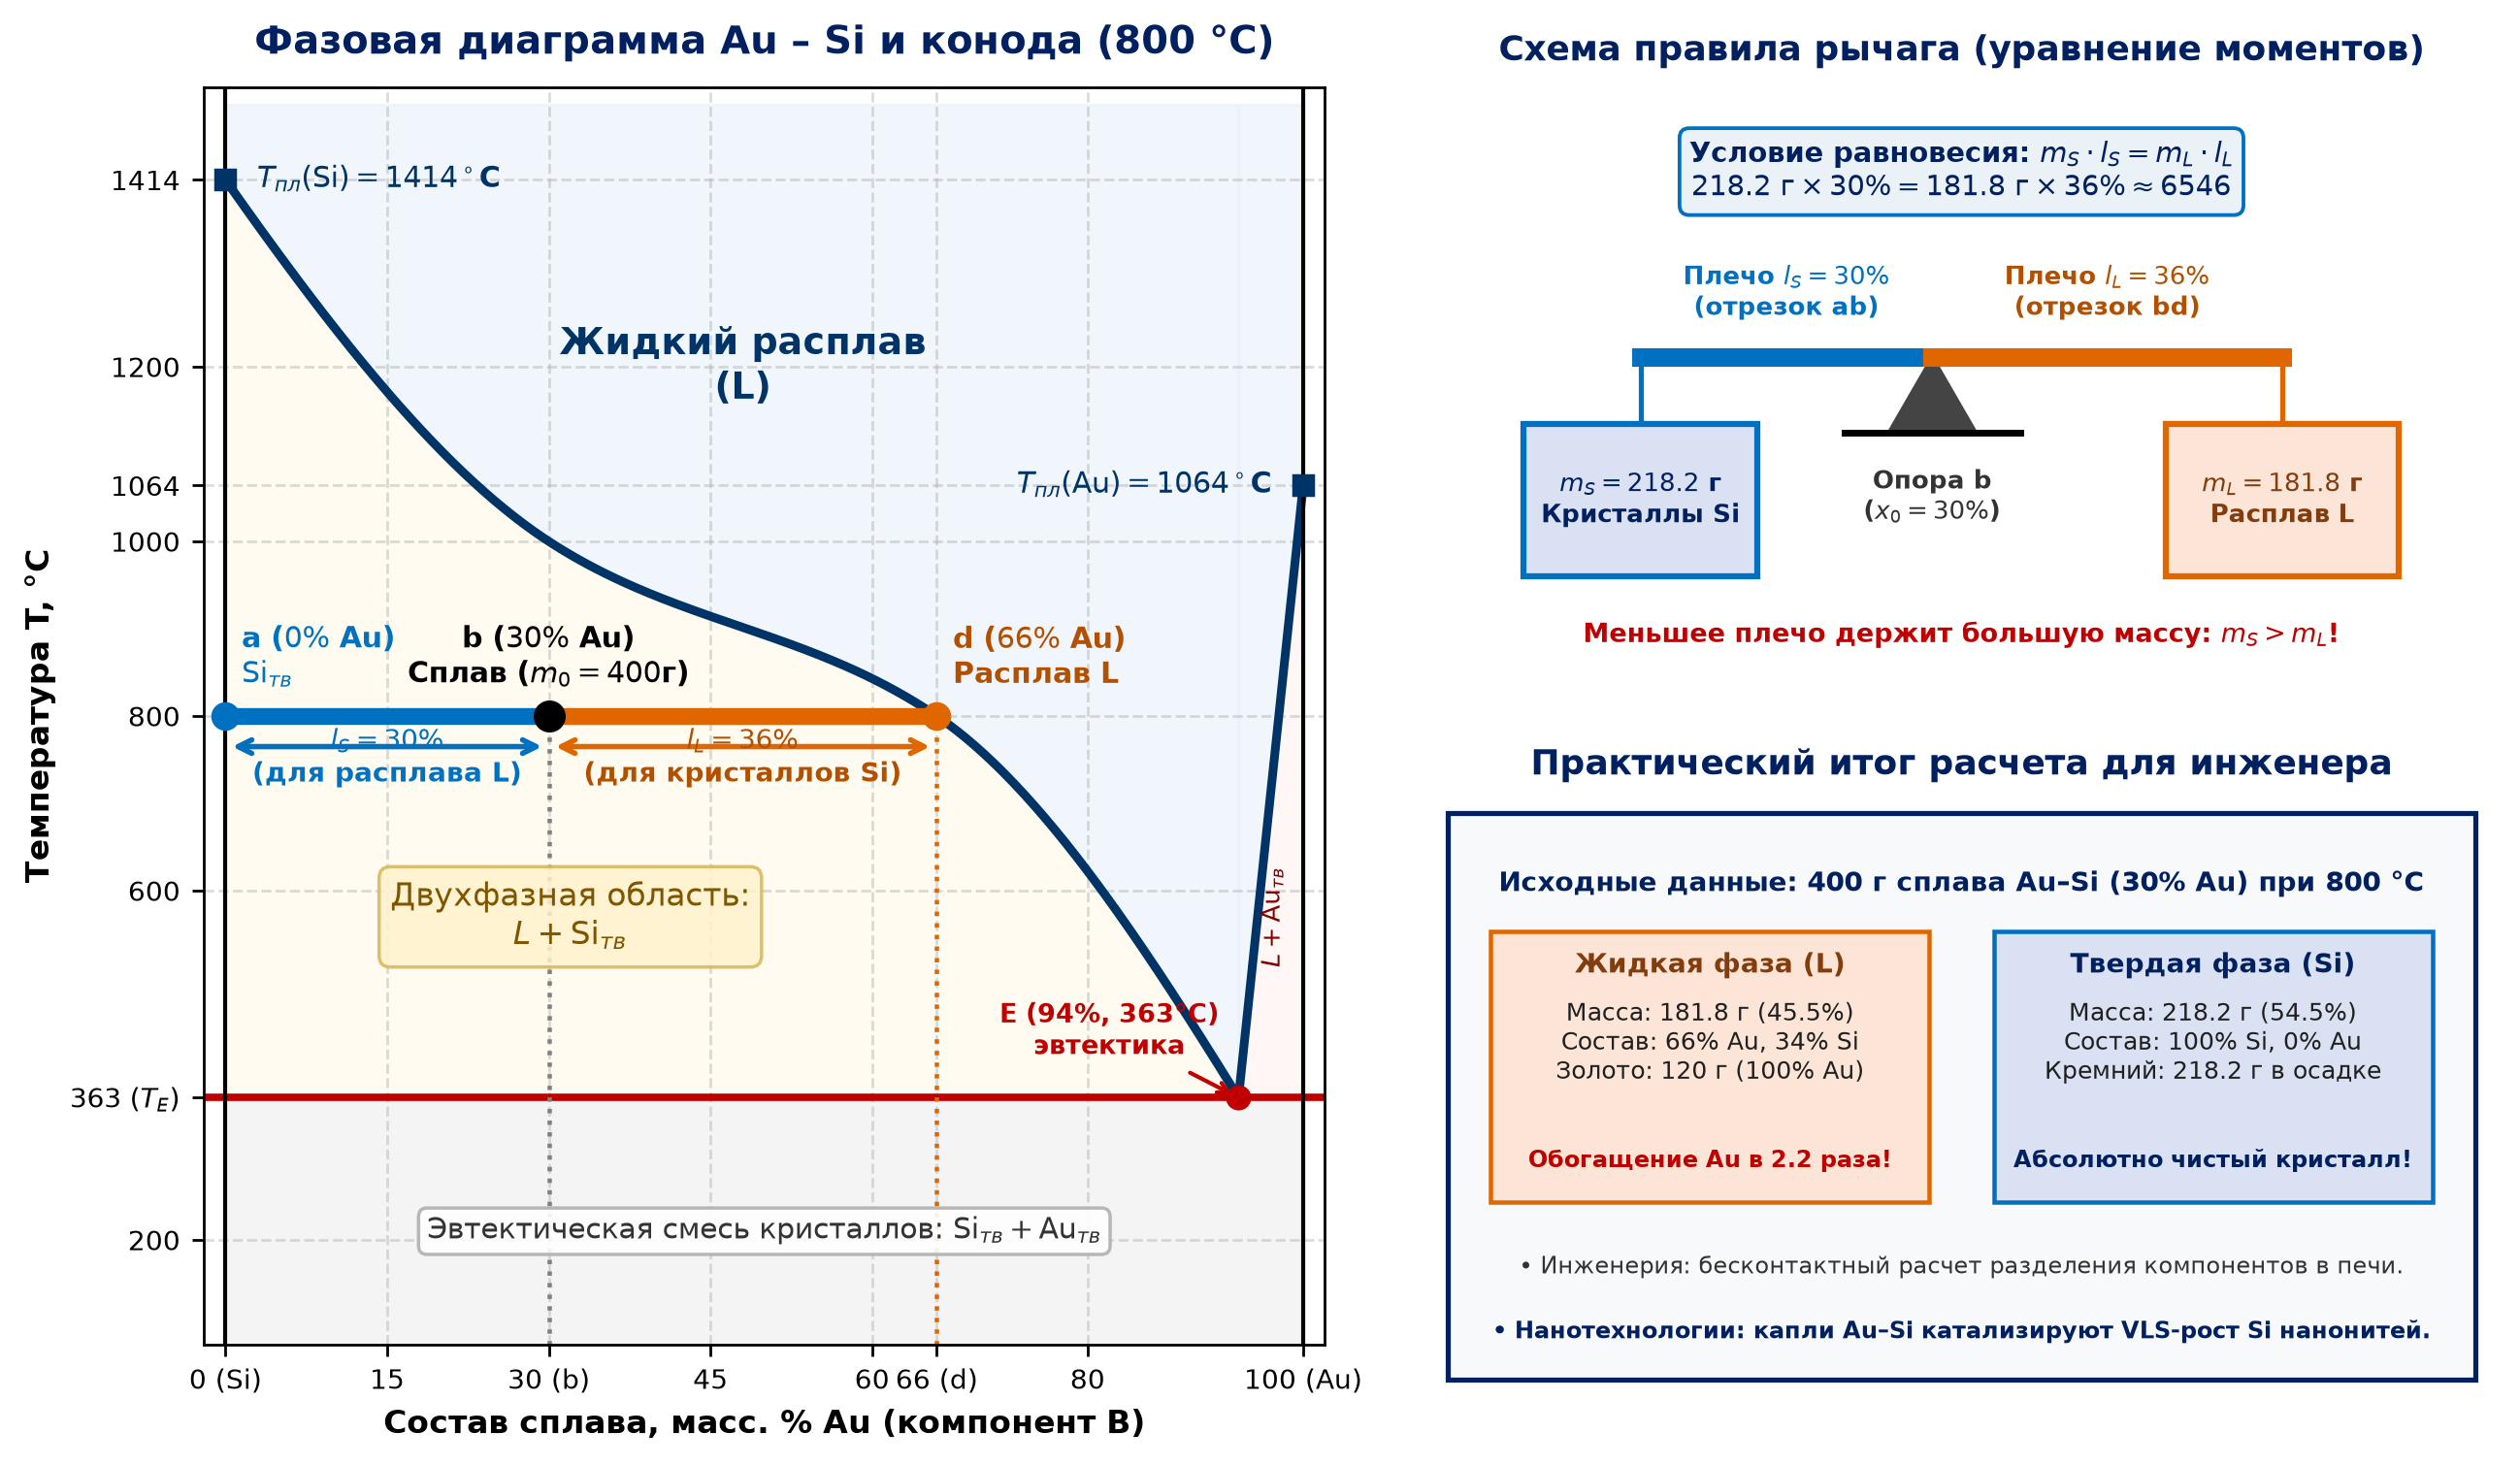
\includegraphics[width=0.92\textwidth]{fig_lever_anatomy.png}
    \caption{Геометрическая анатомия правила рычага для бинарной системы $\mathrm{Au\text{--}Si}$: коннода при $T = 600^\circ\mathrm{C}$, определение составов равновесных фаз по проекциям концов конноды ($C_L$ и $C_S$) и расчет массовых долей расплава $W_L$ и кристаллов $W_S$ по обратно-пропорциональным плечам $l_L$ и $l_S$.}
    \label{fig:lever_anatomy}
\end{figure}

Пусть общий состав сплава задан мольной (или массовой) долей кремния $C_0$. При температуре $T$ коннода пересекает линию ликвидуса в точке $L$ с составом $C_L$ и границу твердой фазы в точке $S$ с составом $C_S$. Обозначим долю жидкой фазы через $W_L$, а долю твердой фазы через $W_S$. 

Уравнения материального баланса имеют вид:
\begin{align}
W_L + W_S &= 1, \label{eq:balance_total}\\
W_L \cdot C_L + W_S \cdot C_S &= C_0. \label{eq:balance_component}
\end{align}
Подставляя $W_L = 1 - W_S$ в уравнение~(\ref{eq:balance_component}):
\begin{equation}
(1 - W_S) C_L + W_S C_S = C_0 \implies W_S (C_S - C_L) = C_0 - C_L.
\end{equation}
Отсюда получаем формулу для доли твердой фазы:
\begin{equation}
W_S = \frac{C_0 - C_L}{C_S - C_L} = \frac{l_L}{l_{\mathrm{total}}}.
\label{eq:lever_ws}
\end{equation}
Аналогично, подставляя $W_S = 1 - W_L$:
\begin{equation}
W_L = \frac{C_S - C_0}{C_S - C_L} = \frac{l_S}{l_{\mathrm{total}}},
\label{eq:lever_wl}
\end{equation}
где $l_L = C_0 - C_L$ --- длина отрезка конноды, прилегающего к фазе жидкости; $l_S = C_S - C_0$ --- длина отрезка конноды, прилегающего к твердой фазе; $l_{\mathrm{total}} = C_S - C_L$ --- полная длина конноды.

\begin{lawbox}{Правило рычага (правило отрезков)}
\begin{enumerate}
    \item \textbf{Составы равновесных фаз} определяются проекциями концов конноды на ось концентраций ($C_L$ и $C_S$).
    \item \textbf{Относительные доли фаз} обратно пропорциональны отрезкам конноды, прилегающим к соответствующим фазам:
    \begin{equation}
    \frac{W_L}{W_S} = \frac{l_S}{l_L} = \frac{C_S - C_0}{C_0 - C_L}.
    \label{eq:lever_ratio}
    \end{equation}
    Доля фазы пропорциональна длине \textbf{противоположного плеча} рычага!
\end{enumerate}
\end{lawbox}

\subsection{Динамика охлаждения сплава по точкам (Точки 1 $\to$ 2 $\to$ 3 $\to$ 4)}
На рис.~\ref{fig:lever_dynamics} продемонстрирована пошаговая эволюция сплава $\mathrm{Au\text{--}30\%\,Si}$ в процессе медленного равновесного охлаждения:

\begin{figure}[htbp]
    \centering
    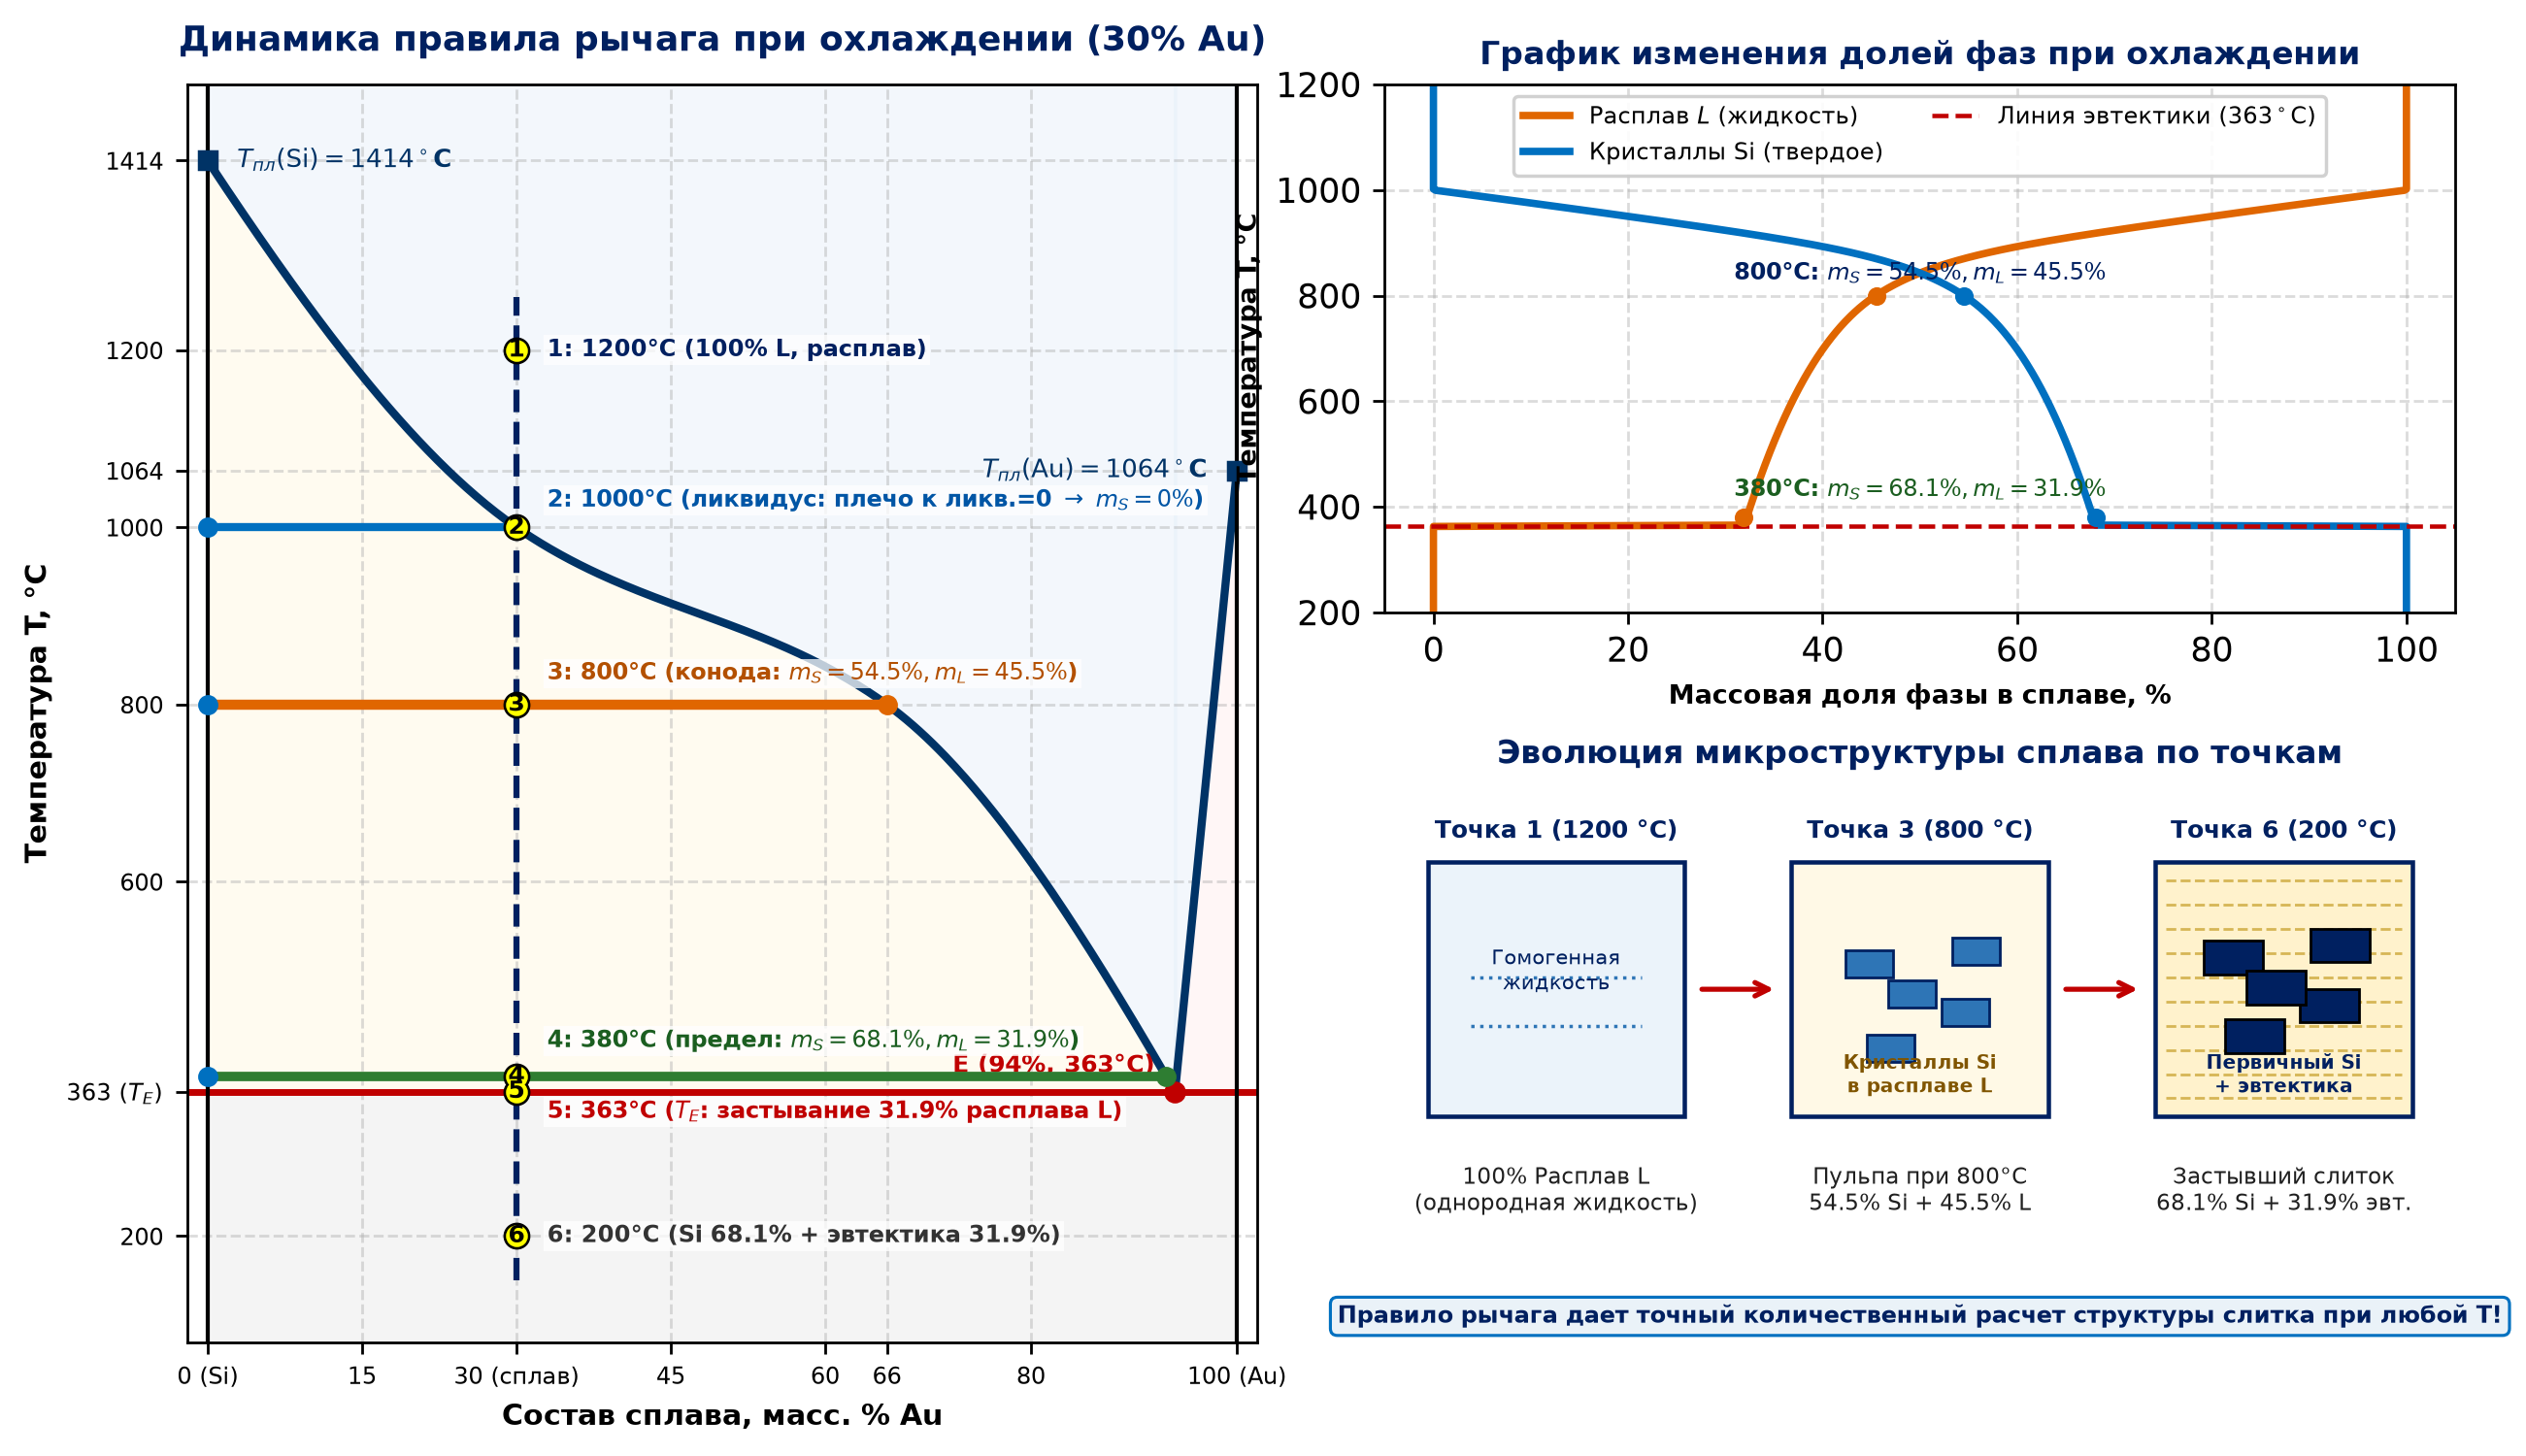
\includegraphics[width=0.92\textwidth]{fig_lever_cooling_dynamics.png}
    \caption{Пошаговый расчет правила рычага в динамике охлаждения сплава $\mathrm{Au\text{--}30\text{ ат. }\%\,Si}$ от расплава до эвтектической кристаллизации: Точка~1 ($1200^\circ\mathrm{C}$, гомогенный расплав) $\to$ Точка~2 ($770^\circ\mathrm{C}$, точка ликвидуса, зарождение первых кристаллов $\mathrm{Si}$) $\to$ Точка~3 ($600^\circ\mathrm{C}$, двухфазная область) $\to$ Точка~4 ($363^\circ\mathrm{C}$, эвтектика).}
    \label{fig:lever_dynamics}
\end{figure}

\begin{itemize}
    \item \textbf{Точка 1 ($T_1 = 1200^\circ\mathrm{C}$):} система находится высоко над линией ликвидуса. Состояние однофазное --- гомогенный жидкий раствор золота и кремния. $W_L = 100\%$, $W_S = 0\%$.
    \item \textbf{Точка 2 ($T_2 \approx 770.2^\circ\mathrm{C}$):} фигуративная точка сплава попадает точно на линию ликвидуса кремния. В этот момент начинается выпадение первых бесконечно малых зародышей твердого кремния. 
    \textit{Физический и геометрический смысл правила рычага в Точке 2:} фигуративная точка совпадает с левым концом конноды. Противоположное твердой фазе плечо $l_S = C_0 - C_L = 30\% - 30\% = 0$. Следовательно:
    \begin{equation*}
    W_S = \frac{l_L}{l_{\mathrm{total}}} = \frac{0}{100\% - 30\%} = 0\%, \qquad W_L = 100\%.
    \end{equation*}
    Твердая фаза только начинает рождаться, ее массовая доля строго равна нулю.
    \item \textbf{Точка 3 ($T_3 = 600^\circ\mathrm{C}$):} система остыла на $170^\circ\mathrm{C}$ ниже ликвидуса. Жидкость обедняется кремнием, ее состав скользит по ликвидусу влево и достигает $C_L = 17.5\text{ ат. }\%\text{ Si}$. Твердая фаза представляет собой чистый кремний ($C_S = 100\text{ ат. }\%\text{ Si}$). Длины плеч составляют:
    \begin{align*}
    l_L &= C_0 - C_L = 30\% - 17.5\% = 12.5\%,\\
    l_S &= C_S - C_0 = 100\% - 30\% = 70.0\%,\\
    l_{\mathrm{total}} &= 100\% - 17.5\% = 82.5\%.
    \end{align*}
    Доля жидкого расплава: $W_L = \frac{70.0}{82.5} \approx 84.8\%$. Доля выделившихся монокристаллов кремния: $W_S = \frac{12.5}{82.5} \approx 15.2\%$.
    \item \textbf{Точка 4 ($T_4 = 363^\circ\mathrm{C} + \varepsilon$):} непосредственно перед эвтектической кристаллизацией жидкая фаза достигла эвтектического состава $C_E = 18.6\text{ ат. }\%\text{ Si}$. Ее доля составляет:
    \begin{equation*}
    W_L = \frac{100 - 30}{100 - 18.6} = \frac{70}{81.4} \approx 86.0\%, \qquad W_S(\text{первичный Si}) = 14.0\%.
    \end{equation*}
    При переходе через $363^\circ\mathrm{C}$ весь оставшийся объем расплава ($86\%$) мгновенно кристаллизуется в тонкодисперсную эвтектическую колонию $(\mathrm{Au} + \mathrm{Si})$.
\end{itemize}

\subsection{Сравнение трех типов сплавов и микроструктура}
В зависимости от исходной концентрации компонентов различают три класса сплавов (рис.~\ref{fig:alloys_comparison}):
\begin{enumerate}
    \item \textbf{Доэвтектические сплавы ($C_0 < C_E = 18.6\text{ ат. }\%\text{ Si}$):} первично кристаллизуются избыточные зерна чистого золота $\alpha(\mathrm{Au})$. Жидкость обогащается кремнием до эвтектики. Итоговая микроструктура: крупные первичные дендриты золота, окруженные мелкодисперсной эвтектикой.
    \item \textbf{Эвтектический сплав ($C_0 = C_E = 18.6\text{ ат. }\%\text{ Si}$):} жидкий расплав кристаллизуется при $T_E = 363^\circ\mathrm{C}$ без первичного выделения фаз. Микроструктура представляет собой $100\%$ однородную тонкую пластинчатую или стержневую эвтектическую колонию.
    \item \textbf{Заэвтектические сплавы ($C_0 > C_E$):} первично выделяются твердые граненые кристаллы кремния $\beta(\mathrm{Si})$. Остаточная жидкость затвердевает в эвтектику.
\end{enumerate}

\begin{figure}[htbp]
    \centering
    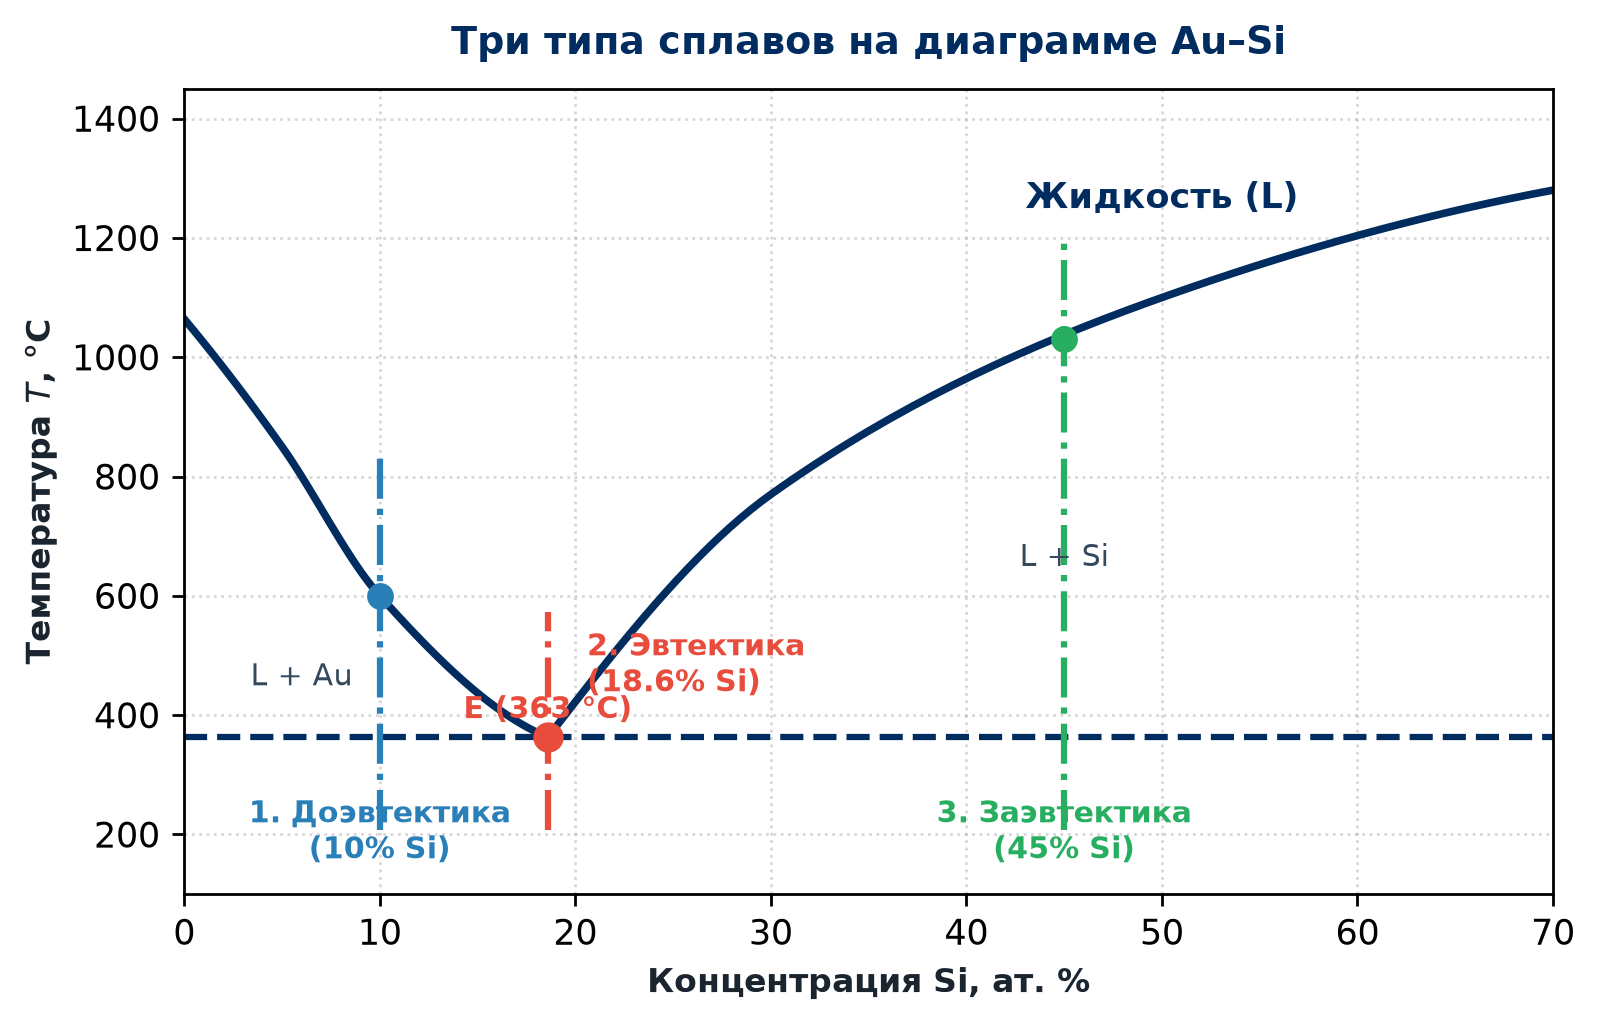
\includegraphics[width=0.88\textwidth]{fig_alloys_comparison.png}
    \caption{Классификация бинарных сплавов на диаграмме состояния $\mathrm{Au\text{--}Si}$: доэвтектический состав 10\% Si (первичные зерна золота), эвтектический состав 18.6\% Si (100\% тонкодисперсная эвтектика) и заэвтектический состав 45\% Si (первичные кристаллы кремния).}
    \label{fig:alloys_comparison}
\end{figure}

\begin{notebox}{Технологическое значение эвтектики Au--Si в микроэлектронике}
Чистое золото плавится при $1064^\circ\mathrm{C}$, а кремний --- при $1414^\circ\mathrm{C}$. Однако их эвтектический сплав плавится при температуре всего \textbf{$363^\circ\mathrm{C}$}! Это явление лежит в основе классической технологии \textbf{эвтектической пайки кристаллов}: кремниевый процессорный чип монтируется на позолоченную подложку корпуса интегральной схемы при умеренном нагреве ($\approx 380^\circ\mathrm{C}$). Образующийся на границе микрослой жидкой эвтектики обеспечивает идеальный электрический и тепловой контакт без риска термического разрушения тончайших $p\text{--}n$ переходов полупроводника.
\end{notebox}

% ==============================================================================
% 2.6. Термодинамика наномасштаба
% ==============================================================================
\section{Термодинамика наномасштаба: поверхностная энергия и зародышеобразование}
\label{sec:nanoscale}

При уменьшении размеров объектов до единиц и десятков нанометров ($1\text{--}100\text{ нм}$) классическая термодинамика массивных тел претерпевает радикальную модификацию. Причиной тому служит \textbf{масштабный фактор}.

\subsection{Вклад поверхности и поверхностное натяжение}
Для сферической частицы радиуса $R$ отношение площади поверхности к объему составляет:
\begin{equation}
\frac{A}{V} = \frac{4\pi R^2}{\frac{4}{3}\pi R^3} = \frac{3}{R}.
\label{eq:surface_to_volume}
\end{equation}
Для макроскопического образца ($R \approx 1\text{ см} = 10^{-2}\text{ м}$) доля атомов, находящихся на поверхности, составляет исчезающе малую величину $\sim 10^{-7}\%$. Однако для наночастицы диаметром $2\text{--}3\text{ нм}$ более $50\text{--}70\%$ всех атомов лежат на границе раздела фаз!

\begin{figure}[htbp]
    \centering
    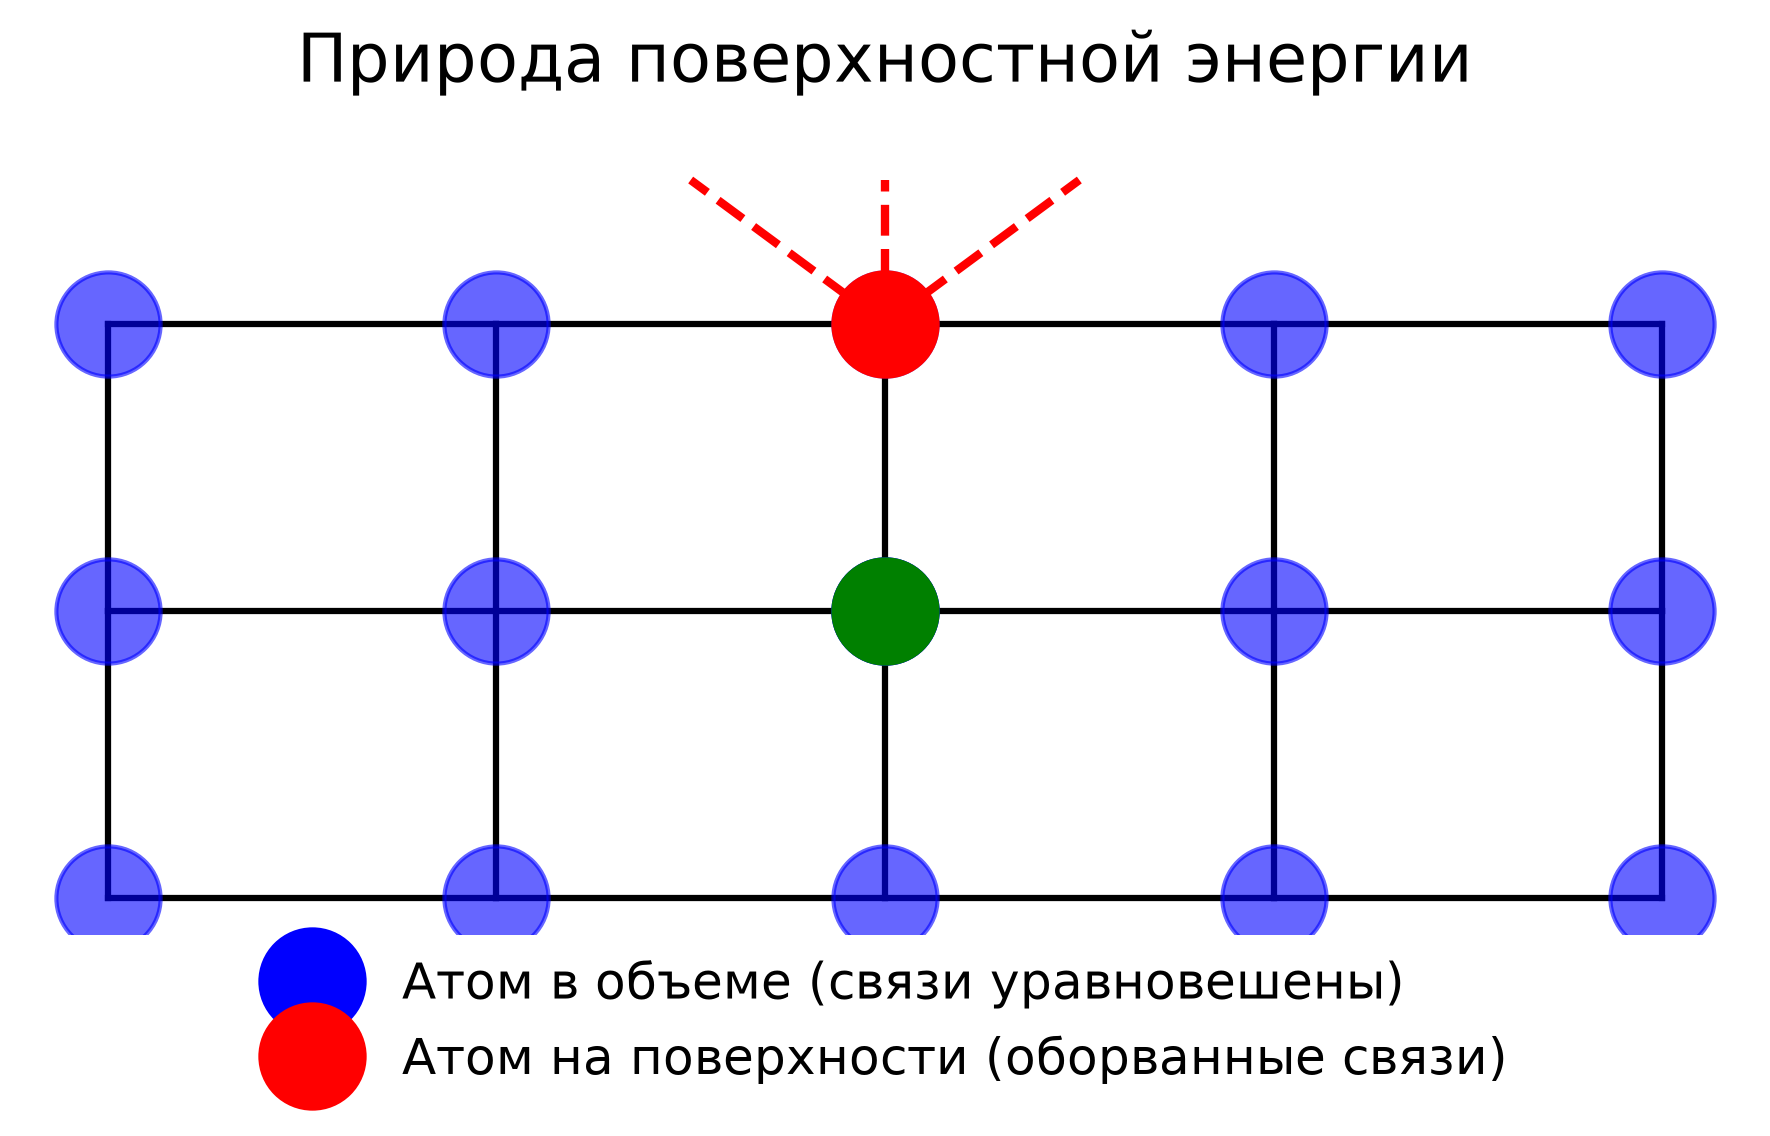
\includegraphics[width=0.82\textwidth]{fig_surface_energy_lattice.png}
    \caption{Микроскопическая природа поверхностной энергии: атом в объеме окружен соседями (связи полностью скомпенсированы); атом на поверхности имеет ненасыщенные (оборванные) химические связи, формирующие избыточную поверхностную энергию $\sigma$.}
    \label{fig:surface_energy}
\end{figure}

Как показано на рис.~\ref{fig:surface_energy}, атом в объеме кристаллической решетки имеет максимальное координационное число: все его связи с соседями скомпенсированы. Атом на поверхности лишен половины соседей --- его химические связи являются «оборванными» (ненасыщенными). Для вывода атома из объема на поверхность необходимо совершить работу против сил межчастичного сцепления. 

Следовательно, создание межфазной поверхности всегда сопряжено с затратами энергии, и основное термодинамическое уравнение Гиббса~(\ref{eq:dg_fundamental}) дополняется поверхностным слагаемым:
\begin{equation}
dG = -S\,dT + V\,dP + \mu\,dN + \sigma\,dA,
\label{eq:dg_with_surface}
\end{equation}
где $\sigma$ --- удельная свободная поверхностная энергия (или коэффициент поверхностного натяжения), выражаемая в $\text{Дж}/\text{м}^2$ или $\text{Н}/\text{м}$; $A$ --- площадь межфазной границы.

\subsection{Термодинамика гомогенного зародышеобразования}
Рассмотрим фазовый переход первого рода (например, кристаллизацию переохлажденного расплава ниже температуры плавления $T_m$). Переход термодинамически выгоден по объему, так как $\mu_{\mathrm{solid}} < \mu_{\mathrm{liquid}}$.

Пусть в глубине расплава флуктуационно зарождается сферический кристаллический кластер радиуса $r$. Изменение энергии Гиббса системы $\Delta G(r)$ складывается из двух конкурирующих членов:
\begin{equation}
\Delta G(r) = \Delta G_V(r) + \Delta G_S(r) = -\frac{4}{3}\pi r^3 \Delta g_v + 4\pi r^2 \sigma,
\label{eq:nucleation_dg}
\end{equation}
где $\Delta g_v = \frac{\Delta H_m \cdot \Delta T}{T_m} > 0$ --- объемная плотность выигрыша свободной энергии при фазовом переходе; $\Delta T = T_m - T$ --- величина переохлаждения; $\Delta H_m$ --- удельная теплота плавления на единицу объема; $\sigma$ --- межфазное натяжение на границе кристалл/расплав.

\begin{figure}[htbp]
    \centering
    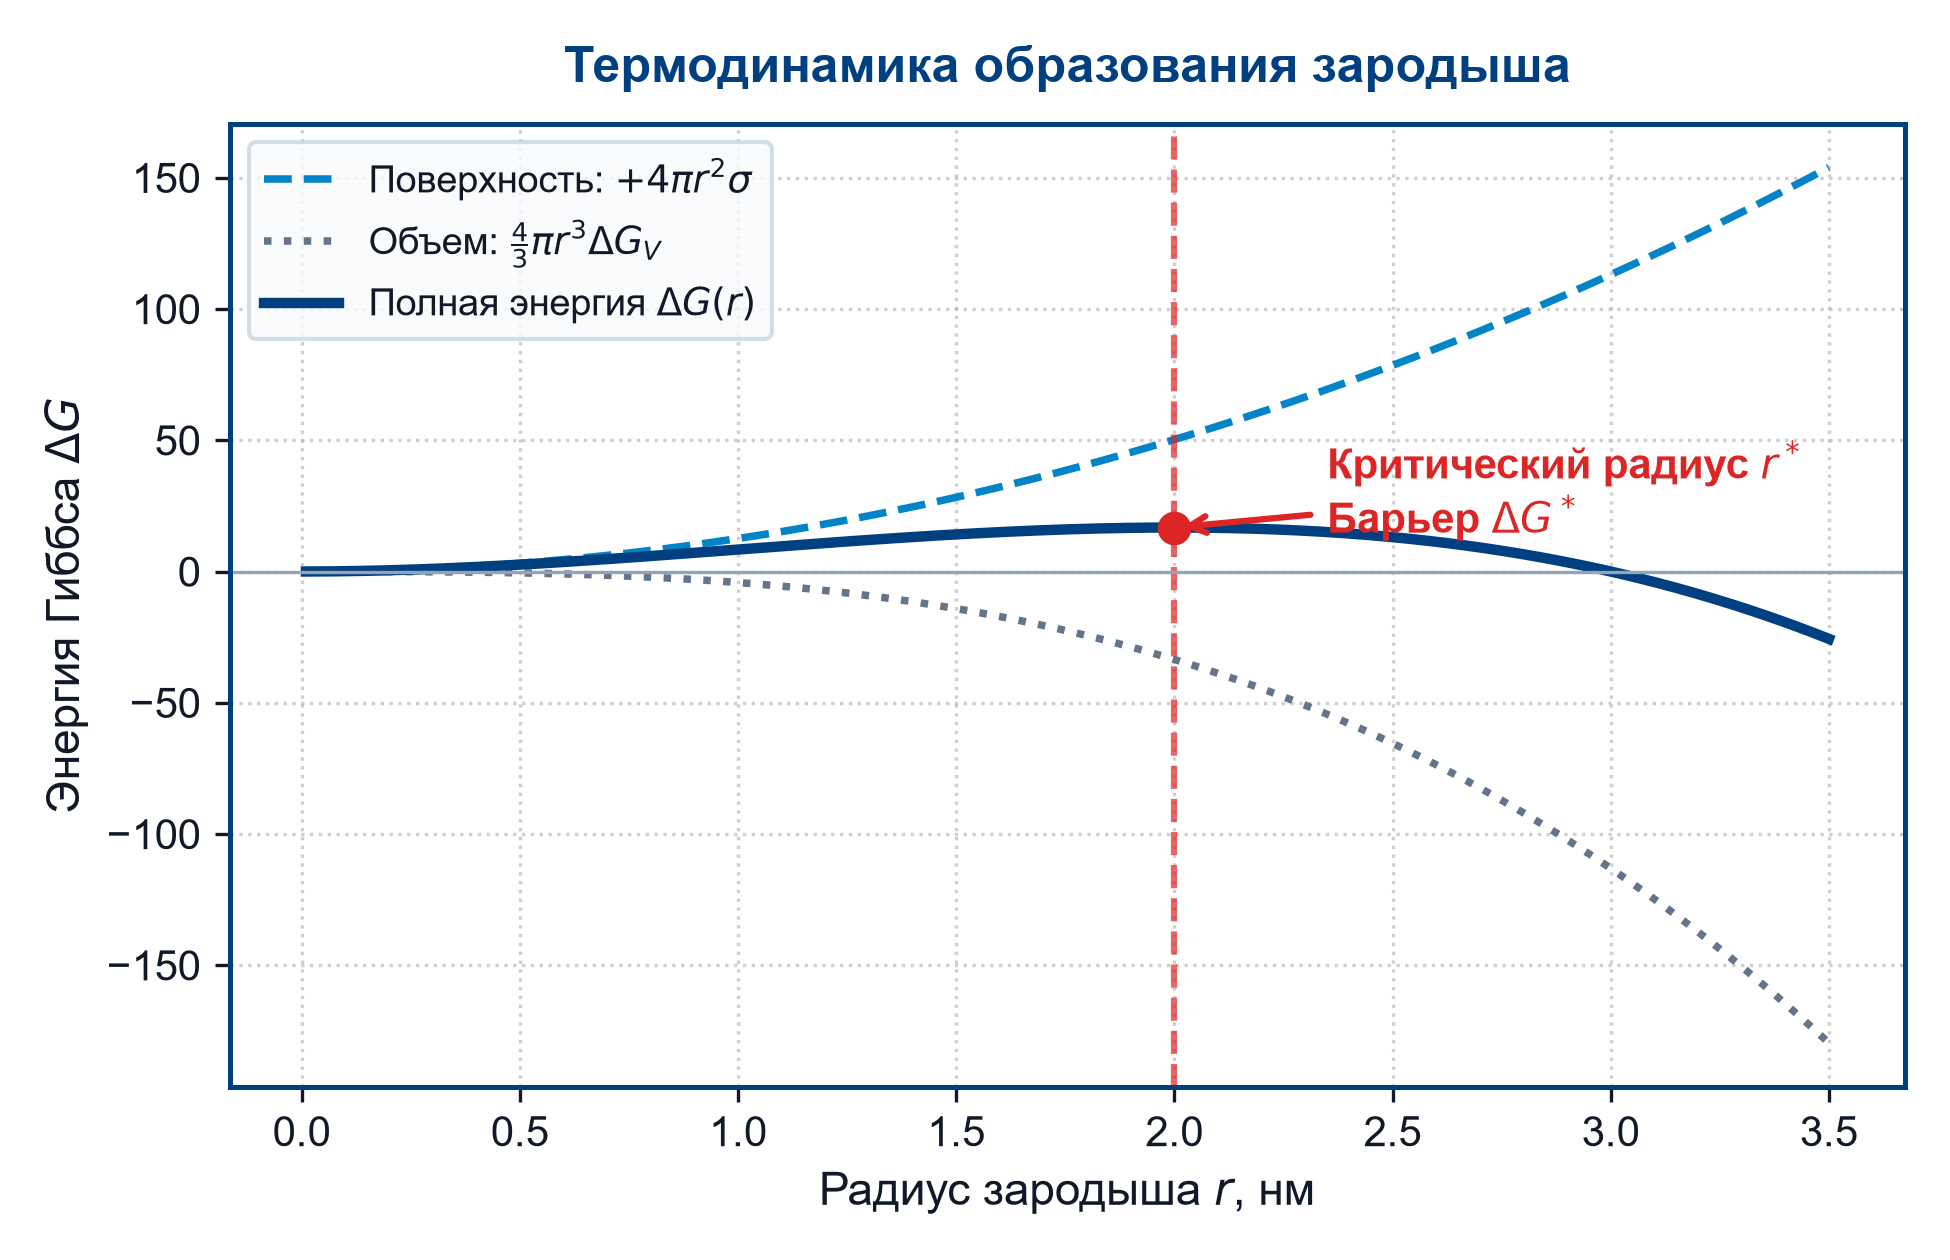
\includegraphics[width=0.88\textwidth]{fig_nucleation_barrier.png}
    \caption{Термодинамика образования зародыша новой фазы: конкуренция объемного выигрыша энергии ($\sim -r^3$) и поверхностных затрат ($\sim +r^2$). Максимум результирующей кривой определяет критический радиус зародыша $r^*$ и высоту термодинамического барьера $\Delta G^*$.}
    \label{fig:nucleation_barrier}
\end{figure}

На рис.~\ref{fig:nucleation_barrier} представлен характер кривой $\Delta G(r)$:
\begin{itemize}
    \item При малых радиусах $r$ квадратичный поверхностный член $4\pi r^2 \sigma$ растет значительно быстрее, чем убывает кубический объемный член $-\frac{4}{3}\pi r^3 \Delta g_v$. Образование субнаноразмерного кластера \textbf{термодинамически невыгодно} ($\Delta G > 0$).
    \item При больших радиусах $r$ кубическая зависимость неизбежно побеждает квадратичную, и свободная энергия устремляется в область глубокого минуса.
\end{itemize}

\subsection{Критический радиус $r^*$ и энергетический барьер $\Delta G^*$}
Для нахождения экстремума продифференцируем $\Delta G(r)$ по радиусу и приравняем производную к нулю:
\begin{equation}
\frac{d \Delta G}{dr} = -4\pi r^2 \Delta g_v + 8\pi r \sigma = 0.
\end{equation}
Отсюда получаем формулу для \textbf{критического радиуса зародыша} $r^*$:
\begin{equation}
r^* = \frac{2\sigma}{\Delta g_v} = \frac{2\sigma T_m}{\Delta H_m \cdot \Delta T}.
\label{eq:r_star}
\end{equation}
Подставляя $r^*$ обратно в выражение~(\ref{eq:nucleation_dg}), находим высоту \textbf{активационного барьера зародышеобразования} $\Delta G^*$:
\begin{equation}
\Delta G^* = -\frac{4}{3}\pi \left(\frac{2\sigma}{\Delta g_v}\right)^3 \Delta g_v + 4\pi \left(\frac{2\sigma}{\Delta g_v}\right)^2 \sigma = \frac{16\pi \sigma^3}{3 (\Delta g_v)^2} = \frac{16\pi \sigma^3 T_m^2}{3 \Delta H_m^2 (\Delta T)^2}.
\label{eq:delta_g_star}
\end{equation}

\begin{lawbox}{Поведение зародышей и технологическое управление}
\begin{itemize}
    \item \textbf{Докритические зародыши ($r < r^*$):} называют \textit{эмбрионами}. Для них $\frac{d\Delta G}{dr} > 0$. Случайно возникнув за счет тепловых флуктуаций, они самопроизвольно растворяются в матрице.
    \item \textbf{Закритические зародыши ($r > r^*$):} преодолели потенциальный барьер ($\frac{d\Delta G}{dr} < 0$). Их дальнейший рост сопровождается непрерывным снижением свободной энергии системы --- они лавинообразно растут, образуя устойчивую фазу.
    \item \textbf{Управление коллоидным синтезом наночастиц:}
    Скорость зародышеобразования подчиняется экспоненциальному закону Аррениуса:
    \begin{equation}
    I = I_0 \exp\left(-\frac{\Delta G^*}{k_B T}\right) = I_0 \exp\left(-\frac{16\pi \sigma^3 T_m^2}{3 k_B T \Delta H_m^2 (\Delta T)^2}\right).
    \label{eq:arrhenius_nucleation}
    \end{equation}
    При создании глубокого переохлаждения расплава или высокого химического пересыщения раствора ($\Delta T \gg 0$) величина $r^*$ сжимается до долей нанометра, а барьер $\Delta G^*$ падает почти до нуля. В объеме мгновенно вспыхивает гигантское число центров кристаллизации. Если в этот момент ввести поверхностно-активные вещества (ПАВ, стабилизирующие лиганды), они пассивируют поверхность, блокируют диффузионный рост и фиксируют ансамбль ультрадисперсных наночастиц заданного калибра!
\end{itemize}
\end{lawbox}

% ==============================================================================
% 2.7. Размерные термодинамические эффекты
% ==============================================================================
\section{Размерные термодинамические эффекты в наноструктурах}
\label{sec:size_effects}

\subsection{Давление Лапласа и химический потенциал наночастицы}
Искривление границы раздела фаз порождает избыточное капиллярное \textbf{давление Лапласа}:
\begin{equation}
\Delta P = \frac{2\sigma}{r}.
\label{eq:laplace_pressure}
\end{equation}
Для макроскопического шарика ($r = 1\text{ мм}$) давление Лапласа ничтожно ($\Delta P \approx 2\cdot 10^{-3}\text{ атм}$). Но для наночастицы радиусом $r = 1.5\text{ нм}$ при характерном поверхностном натяжении металлов $\sigma \approx 1\text{ Дж}/\text{м}^2$:
\begin{equation*}
\Delta P = \frac{2 \cdot 1.0}{1.5 \cdot 10^{-9}} \approx 1.33 \cdot 10^9\text{ Па} = 1.33\text{ ГПа} \approx 13\,000\text{ атмосфер!}
\end{equation*}
Колоссальное внутреннее давление Лапласа механически сжимает наночастицу и смещает ее химический потенциал относительно массивного плоского кристалла:
\begin{equation}
\mu(r) = \mu_\infty + V_m \Delta P = \mu_\infty + \frac{2\sigma V_m}{r},
\label{eq:chem_pot_curved}
\end{equation}
где $V_m$ --- молярный объем твердой фазы; $\mu_\infty$ --- химический потенциал массивного образца.

\subsection{Размерная зависимость температуры плавления (уравнение Гиббса--Томсона)}
Повышение химического потенциала атомов наночастицы приводит к фундаментальному термодинамическому эффекту: \textbf{температура плавления наночастиц падает при уменьшении их радиуса}.

Приравняем химический потенциал твердой наночастицы $\mu_s(r, T)$ и жидкого расплава $\mu_l(T)$ вблизи точки плавления. Разлагая потенциалы в ряд Тейлора по температуре около температуры плавления массивного материала $T_{m,\infty}$, получаем классическое \textbf{уравнение Гиббса--Томсона}:
\begin{equation}
T_m(r) = T_{m,\infty} \left( 1 - \frac{2\sigma_{sl}}{\rho_s \Delta H_m \, r} \right),
\label{eq:gibbs_thomson}
\end{equation}
где $\sigma_{sl}$ --- межфазное натяжение границы раздела «твердое/жидкость»; $\rho_s$ --- плотность твердой фазы; $\Delta H_m$ --- удельная теплота плавления ($\text{Дж}/\text{кг}$).

\begin{figure}[htbp]
    \centering
    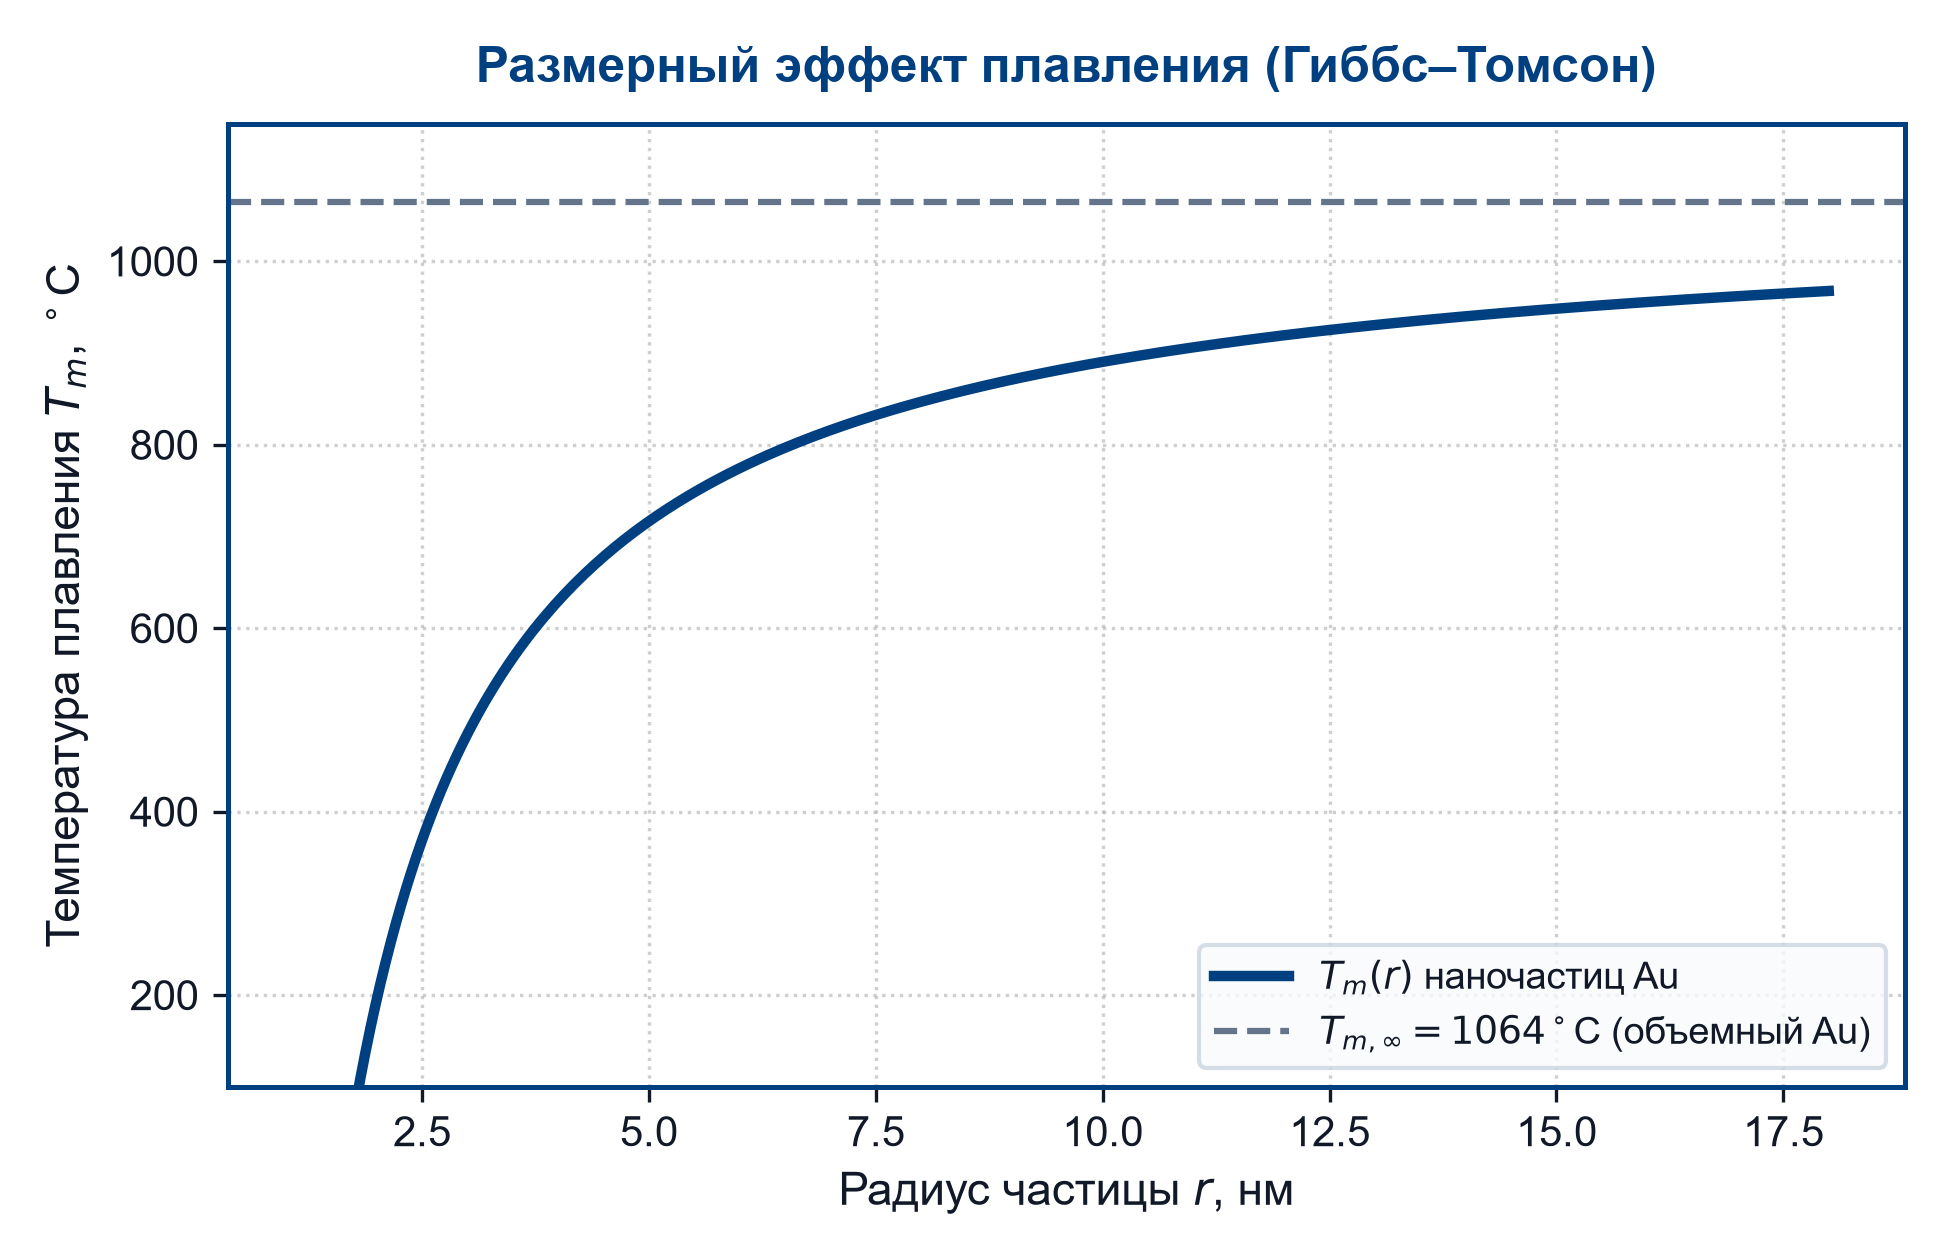
\includegraphics[width=0.88\textwidth]{fig_gibbs_thomson_au.png}
    \caption{Размерный эффект плавления: теоретическая кривая Гиббса--Томсона для наночастиц золота в сравнении с температурой плавления массивного золота $T_{m,\infty} = 1064^\circ\mathrm{C}$ (экспериментальные данные Ph.~Buffat and J.-P.~Borel).}
    \label{fig:gibbs_thomson}
\end{figure}

На рис.~\ref{fig:gibbs_thomson} представлена зависимость $T_m(r)$ для золота. Массивное золото плавится при температуре $1064^\circ\mathrm{C}$. Для частиц радиусом $5\text{ нм}$ температура плавления снижается до $950^\circ\mathrm{C}$, а при $r \le 2\text{ нм}$ температура плавления падает катастрофически --- до $350\text{--}400^\circ\mathrm{C}$!

\begin{notebox}{Физический механизм поверхностного предплавления}
С микроскопической точки зрения плавление наночастицы начинается не во всем объеме, а с ее поверхности (surface premelting). Из-за оборванных связей среднеквадратичная амплитуда тепловых колебаний поверхностных атомов $\langle u^2 \rangle$ оказывается в $2\text{--}3$ раза выше, чем в глубине решетки. Поэтому классический критерий плавления Линдемана (колебания превышают $\approx 10\%$ межатомного расстояния) выполняется на поверхности на сотни градусов раньше, чем в ядре. Наночастица покрывается квазижидкой оболочкой толщиной $1\text{--}2$ монослоя задолго до полного расплавления.
\end{notebox}

\subsection{Размерная модификация фазовых диаграмм: наноэвтектика}
Поскольку температура плавления $T_m(r)$ зависит от радиуса наночастиц, фундаментальный вывод гласит: \textbf{в наномире фазовая диаграмма перестает быть универсальной константой вещества и становится функцией размера $r$!}

\begin{figure}[htbp]
    \centering
    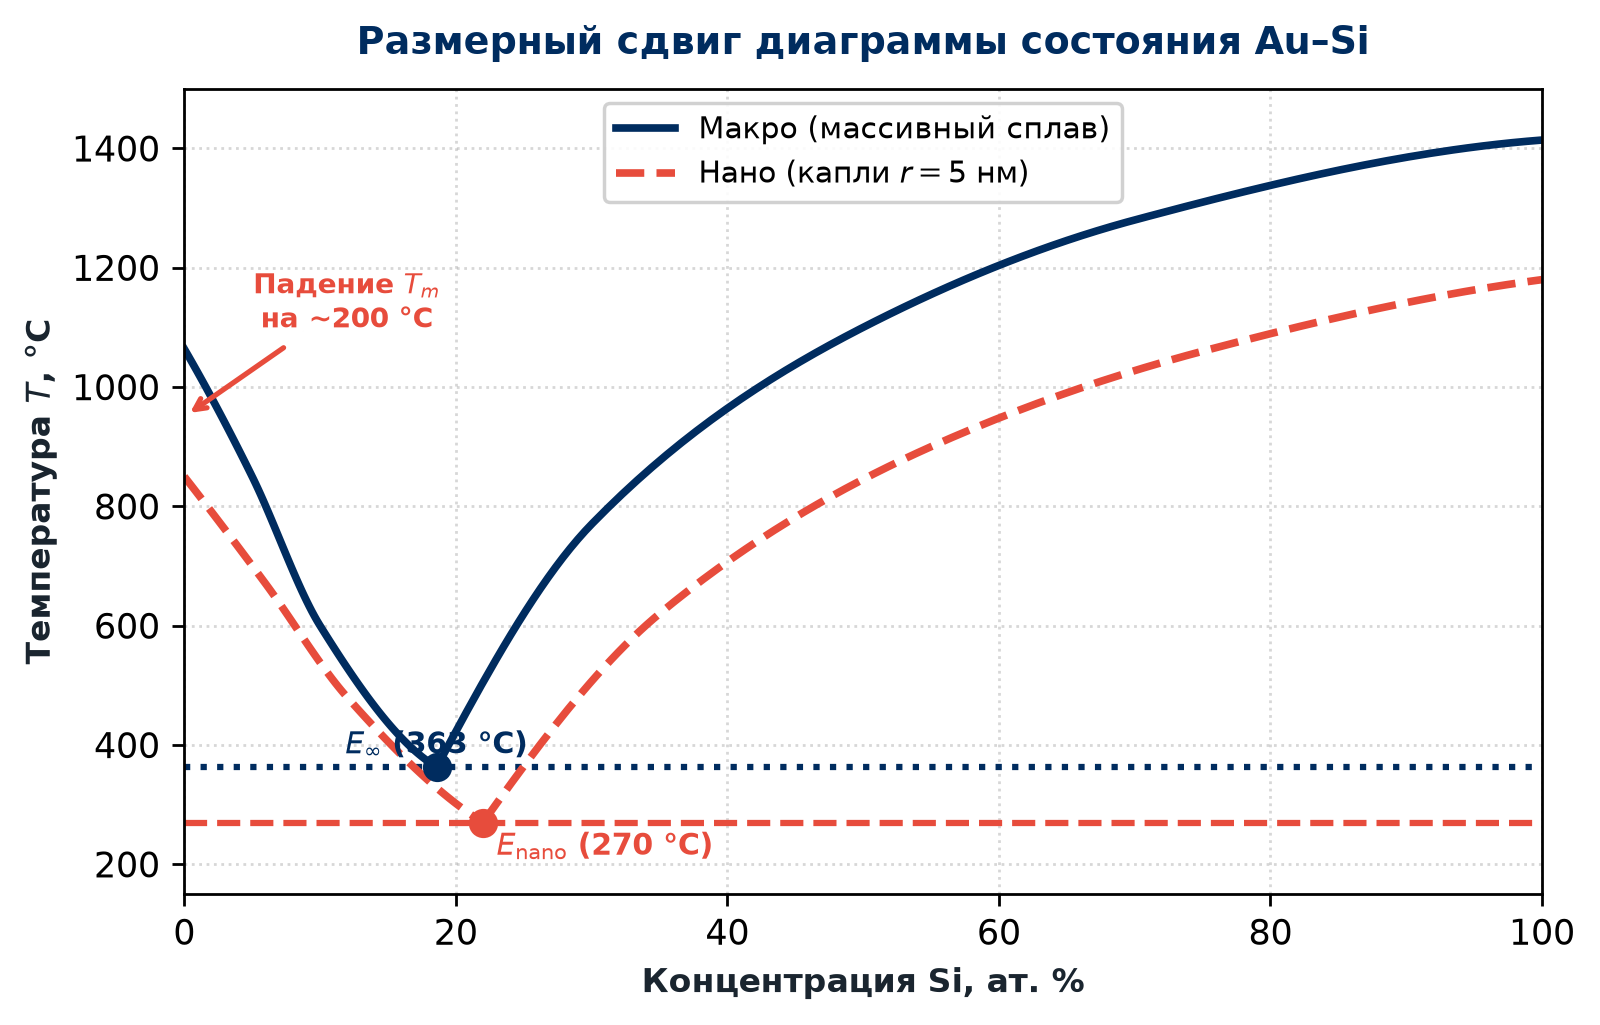
\includegraphics[width=0.88\textwidth]{fig_nano_eutectic_shift.png}
    \caption{Модификация фазовой диаграммы бинарной системы $\mathrm{Au\text{--}Si}$ в наномасштабе: сплошные темно-синие линии --- макроскопический сплав ($E_\infty = 363^\circ\mathrm{C}$); пунктирные красные линии --- нанокапли радиуса $r = 5\text{ нм}$ ($E_{\mathrm{nano}} \approx 270^\circ\mathrm{C}$, сдвиг эвтектической точки вниз и вправо).}
    \label{fig:nano_eutectic}
\end{figure}

На рис.~\ref{fig:nano_eutectic} показана деформация фазовой диаграммы $\mathrm{Au\text{--}Si}$ при переходе к нанокаплям катализатора $r = 5\text{ нм}$:
\begin{enumerate}
    \item \textbf{Снижение эвтектической температуры ($T_E(r) < T_E(\infty)$):} температура эвтектического плавления падает с $363^\circ\mathrm{C}$ до $\approx 270^\circ\mathrm{C}$.
    \item \textbf{Асимметричный дрейф эвтектической концентрации ($C_E(r)$):} поверхностные натяжения золота и кремния различны ($\sigma_{\mathrm{Au}} \ne \sigma_{\mathrm{Si}}$), поэтому ветви ликвидуса опускаются с разной скоростью. Точка эвтектики дрейфует в сторону кремния (с $18.6\%$ до $\approx 22\text{ ат. }\%$).
    \item \textbf{Расширение пределов взаимной растворимости:} в ультрадисперсном состоянии растворимость компонентов возрастает в несколько раз по сравнению с макрокристаллами.
    \item \textbf{Стабилизация метастабильных фаз:} фазы, термодинамически запрещенные в объеме при нормальных условиях, могут стать стабильными в наночастицах, если их удельная поверхностная энергия ниже (классический пример --- стабилизация тетрагональной фазы диоксида циркония $\mathrm{ZrO}_2$ при $20^\circ\mathrm{C}$ только в нанозернах размером менее $30\text{ нм}$).
\end{enumerate}

% ==============================================================================
% 2.8. Технологическое применение: VLS-механизм
% ==============================================================================
\section{Технологическое применение: VLS-механизм направленного роста нанопроволок}
\label{sec:vls}

Прямым триумфом практического применения нанотермодинамики эвтектической системы $\mathrm{Au\text{--}Si}$ является открытый Вагнером и Эллисом механизм \textbf{«Пар--Жидкость--Кристалл»} (Vapor--Liquid--Solid, VLS-механизм) для прецизионного выращивания монокристаллических кремниевых нанопроволок (nanowires).

\begin{figure}[htbp]
    \centering
    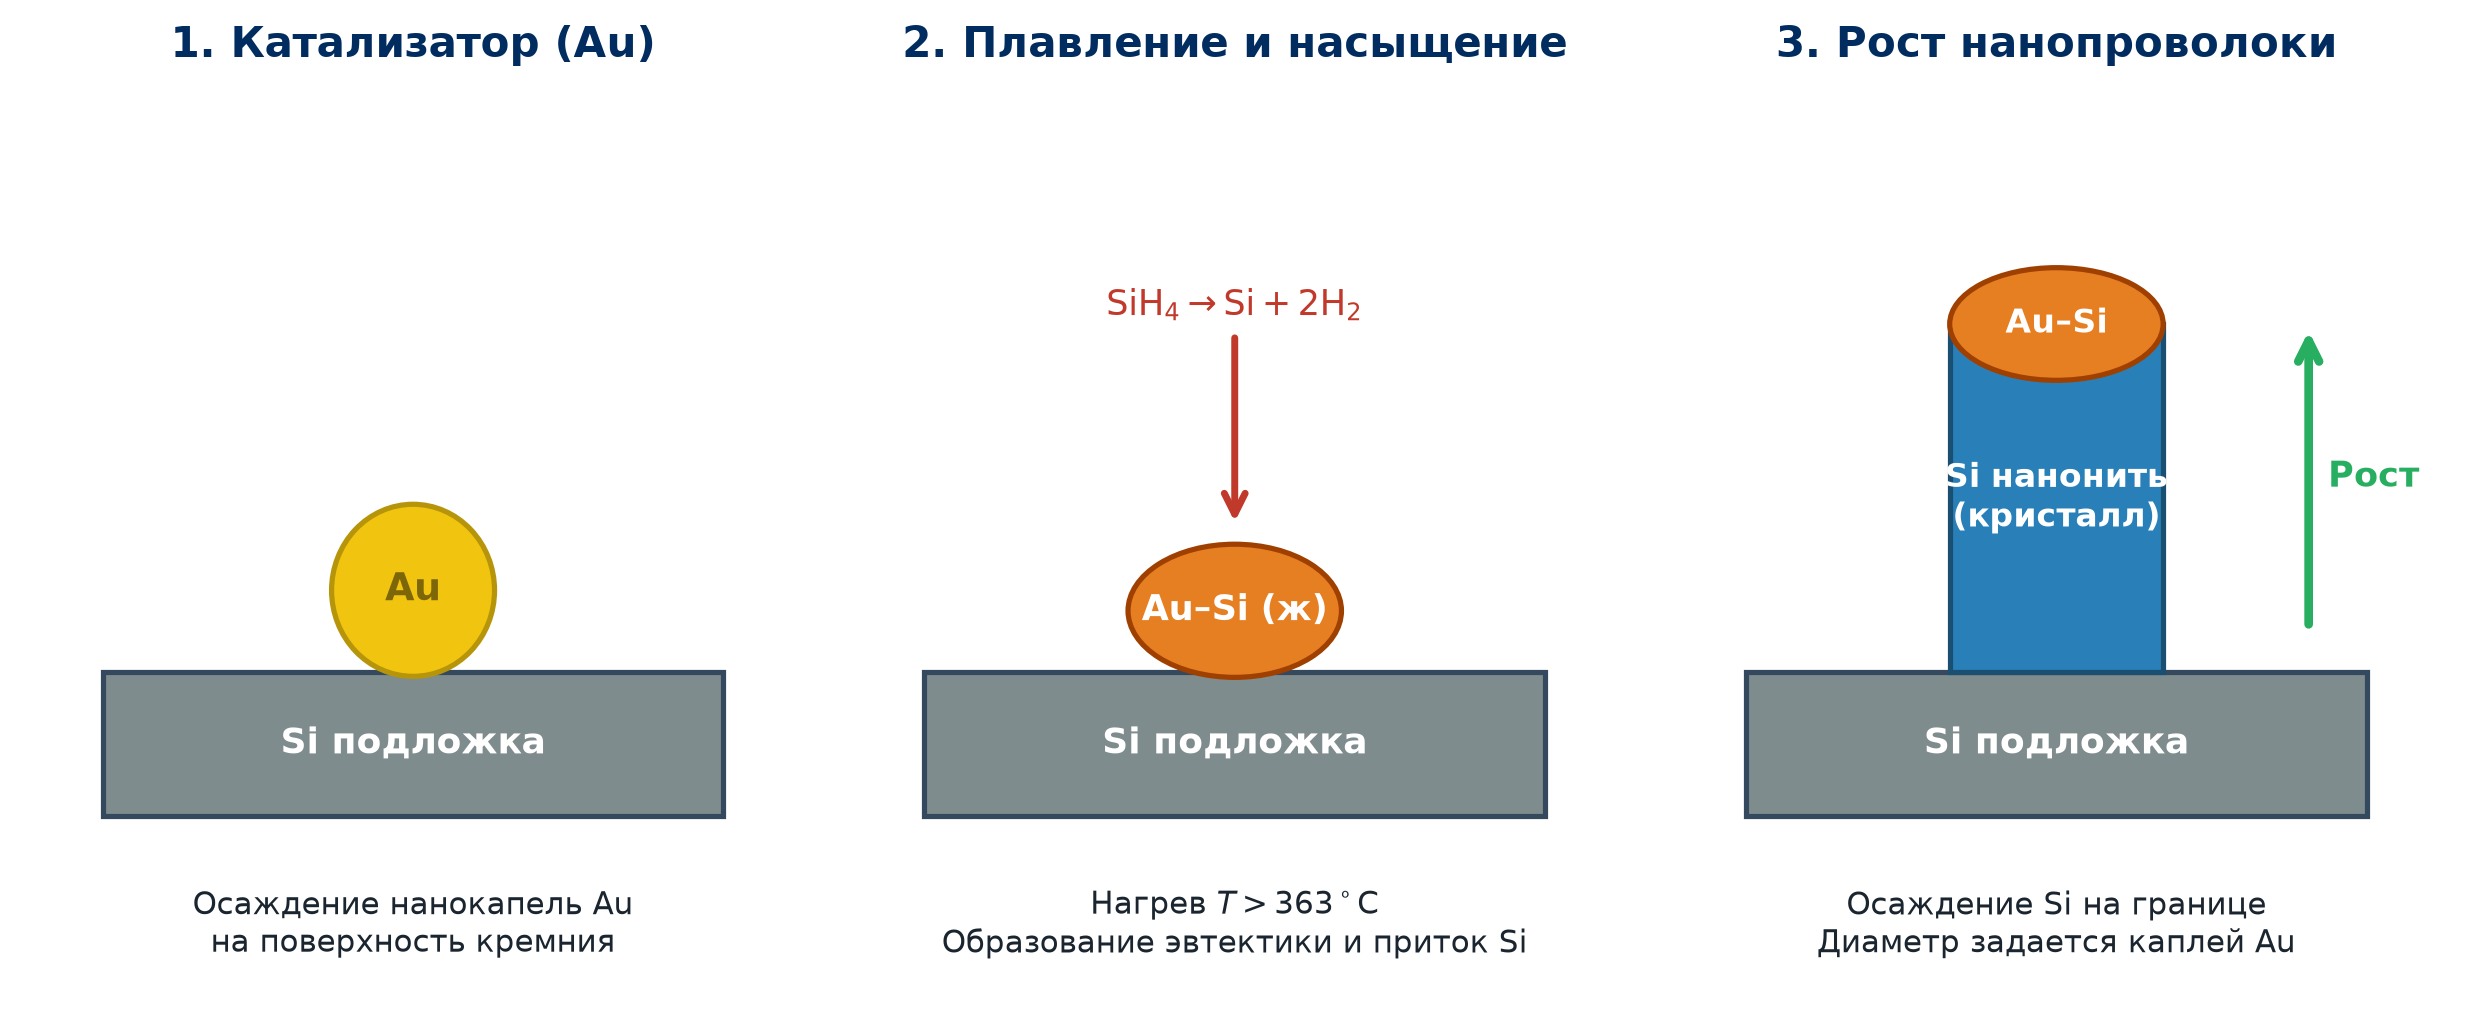
\includegraphics[width=0.92\textwidth]{fig_vls_mechanism_stages.png}
    \caption{Стадии технологического процесса направленного синтеза кремниевых нанопроволок по механизму «Пар--Жидкость--Кристалл» (VLS): (1) нанесение нанокапель катализатора Au; (2) нагрев $T > 363^\circ\mathrm{C}$, образование жидкой эвтектики $\mathrm{Au\text{--}Si}$ и каталитический распад газового прекурсора $\mathrm{SiH}_4$; (3) пересыщение капли и эпитаксиальный рост монокристаллической нанонити кремния под каплей.}
    \label{fig:vls_mechanism}
\end{figure}

Процесс состоит из трех строго контролируемых стадий (рис.~\ref{fig:vls_mechanism}):
\begin{enumerate}
    \item \textbf{Стадия 1 (Осаждение нанокатализатора):} на кремниевую монокристаллическую подложку наносят коллоидные наночастицы золота диаметром $10\text{--}50\text{ нм}$ (или напыляют тончайшую островковую пленку золота).
    \item \textbf{Стадия 2 (Формирование эвтектического расплава и подача газа):} реактор нагревают в вакууме до температуры $T \approx 400\text{--}450^\circ\mathrm{C}$ (выше наноэвтектической точки). Нанокапли золота расплавляются, растворяя кремний подложки до достижения равновесной эвтектической концентрации жидкого сплава $\mathrm{Au\text{--}Si}$.
    В камеру подают газообразный прекурсор кремния --- силан $\mathrm{SiH}_4$. На чистой поверхности твердого кремния силан практически не разлагается, однако жидкая капля золота служит высокоэффективным химическим катализатором:
    \begin{equation}
    \mathrm{SiH}_4\text{ (газ)} \xrightarrow{\mathrm{Au\text{ катализатор}}} \mathrm{Si}\text{ (раств.)} + 2\mathrm{H}_2\uparrow\text{ (газ)}.
    \label{eq:silane_decomposition}
    \end{equation}
    \item \textbf{Стадия 3 (Направленная кристаллизация и рост нити):} непрерывный приток кремния из газовой фазы приводит к пересыщению жидкой капли выше линии ликвидуса ($C_{\mathrm{Si}} > C_{\mathrm{ликвидус}}$). Избыточный кремний термодинамически вынужден кристаллизоваться. Единственной энергетически доступной поверхностью для эпитаксиального осаждения является нижняя граница раздела «жидкая капля / кристаллическая подложка». 
    
    Выделяющийся монокристаллический кремний выстраивает идеальную атомную решетку, поднимая жидкую каплю золота над поверхностью подложки. По мере подачи газа капля «едет» на вершине растущего столбика кремния, формируя идеально гладкую монокристаллическую нанопроволоку.
\end{enumerate}

\begin{lawbox}{Термодинамическая движущая сила VLS-роста}
Движущей силой процесса является ступенчатый градиент химического потенциала кремния:
\begin{equation}
\mu_{\mathrm{Si}}(\text{газ, } \mathrm{SiH}_4) > \mu_{\mathrm{Si}}(\text{жидкая эвтектика } \mathrm{Au\text{--}Si}) > \mu_{\mathrm{Si}}(\text{растущий кристалл } \mathrm{Si}).
\label{eq:vls_driving_force}
\end{equation}
Диаметр получаемой нанонити строго контролируется начальным диаметром нанокапли золота! Сегодня VLS-технология является фундаментальной основой производства транзисторов с круговым затвором (GAAFET) суб-2-нм процессорных топологий и элементов интегральной нанофотоники.
\end{lawbox}

% ==============================================================================
% 2.9. Связь с практикумом
% ==============================================================================
\section{Методическая связь с лабораторным практикумом}
\label{sec:lab_connection}

Изученный термодинамический материал непосредственно готовит студентов к выполнению лабораторных работ 4-го семестра по дисциплине «Физические основы нанотехнологий»:

\begin{enumerate}
    \item \textbf{Лабораторная работа №1 «Оптические и плазмонные свойства металлических наночастиц»:}
    Опирается на размерные эффекты в металлических нанокластерах золота и серебра. Студенты исследуют локализованный поверхностный плазмонный резонанс, спектральное положение которого напрямую зависит от формы, диэлектрического окружения и размера наночастиц, подчиняющегося законам поверхностной термодинамики.
    \item \textbf{Лабораторная работа №2 «Термический анализ и фазовые переходы в наноматериалах»:}
    Практическое воплощение §~\ref{sec:binary_diagrams}. Студенты проводят экспериментальные измерения на дифференциальном сканирующем калориметре (ДСК), регистрируют кривые охлаждения сплавов, определяют температуры ликвидуса, солидуса и скрытые теплоты эвтектических превращений.
    \item \textbf{Лабораторная работа №3 «Коллоидный химический синтез наночастиц»:}
    Прямое моделирование §~\ref{sec:nanoscale}. Регулируя температуру синтеза и концентрацию восстановителя, студенты управляют пересыщением $\Delta g_v$, варьируют критический радиус $r^*$ и оценивают устойчивость наноколлоидов против коагуляции (Оствальдовского созревания).
\end{enumerate}

% ==============================================================================
% 2.10. Примеры решения задач
% ==============================================================================
\section{Примеры решения типовых расчетных задач}
\label{sec:examples}

\begin{exbox}{Задача 1: Расчет фазового состава по правилу рычага}
\textbf{Условие:} Навеска бинарного сплава золото--кремний массой $m_0 = 50\text{ г}$ с концентрацией кремния $C_0 = 30\text{ ат. }\%\text{ Si}$ охлаждена до температуры $T = 600^\circ\mathrm{C}$. По данным фазовой диаграммы (рис.~\ref{fig:lever_anatomy}), состав равновесного жидкого расплава при этой температуре составляет $C_L = 17.5\text{ ат. }\%\text{ Si}$, а твердая фаза представляет собой чистый кремний ($C_S = 100\text{ ат. }\%\text{ Si}$).
Определите:
\begin{enumerate}
    \item Мольные доли жидкой ($W_L$) и твердой ($W_S$) фаз при $600^\circ\mathrm{C}$.
    \item Мольную долю эвтектической смеси ($W_{\text{эвт}}$) после полного охлаждения до комнатной температуры ($C_E = 18.6\text{ ат. }\%\text{ Si}$).
\end{enumerate}

\tcbline
\textbf{Решение:}
\begin{enumerate}
    \item Применим правило рычага~(\ref{eq:lever_ws})--(\ref{eq:lever_wl}) для температуры $600^\circ\mathrm{C}$:
    \begin{align*}
    l_L &= C_0 - C_L = 30.0 - 17.5 = 12.5\text{ ат. }\%,\\
    l_S &= C_S - C_0 = 100.0 - 30.0 = 70.0\text{ ат. }\%,\\
    l_{\mathrm{total}} &= C_S - C_L = 100.0 - 17.5 = 82.5\text{ ат. }\%.
    \end{align*}
    Мольная доля жидкого расплава:
    \begin{equation*}
    W_L = \frac{l_S}{l_{\mathrm{total}}} = \frac{70.0}{82.5} \approx 0.8485 \quad (84.85\%).
    \end{equation*}
    Мольная доля кристаллов кремния:
    \begin{equation*}
    W_S = \frac{l_L}{l_{\mathrm{total}}} = \frac{12.5}{82.5} \approx 0.1515 \quad (15.15\%).
    \end{equation*}
    Проверка: $W_L + W_S = 0.8485 + 0.1515 = 1.000$ ($100\%$).

    \item Для расчета доли эвтектической составляющей в структуре затвердевшего сплава используем баланс для эвтектической точки ($T = 363^\circ\mathrm{C}$):
    \begin{equation*}
    W_{\text{эвт}} = \frac{C_S - C_0}{C_S - C_E} = \frac{100.0 - 30.0}{100.0 - 18.6} = \frac{70.0}{81.4} \approx 0.8599 \quad (86.0\%).
    \end{equation*}
    Доля первичных кристаллов кремния в микроструктуре:
    \begin{equation*}
    W_{\mathrm{Si}}^{\mathrm{prim}} = 1 - W_{\text{эвт}} = 1 - 0.8599 \approx 0.1401 \quad (14.0\%).
    \end{equation*}
\end{enumerate}
\textbf{Ответ:} 1) $W_L \approx 84.85\%$, $W_S \approx 15.15\%$; 2) $W_{\text{эвт}} \approx 86.0\%$, $W_{\mathrm{Si}}^{\mathrm{prim}} \approx 14.0\%$.
\end{exbox}

\begin{exbox}{Задача 2: Расчет критического радиуса зародыша}
\textbf{Условие:} При синтезе нанопорошка кремния из переохлажденного расплава температура плавления чистого кремния составляет $T_m = 1687\text{ К}$ ($1414^\circ\mathrm{C}$), удельная объемная теплота плавления $\Delta H_m = 4.12 \cdot 10^9\text{ Дж}/\text{м}^3$, а удельное межфазное натяжение на границе кристалл/расплав $\sigma = 0.40\text{ Дж}/\text{м}^2$.
Рассчитайте:
\begin{enumerate}
    \item Критический радиус зародыша $r^*$ при переохлаждении расплава на $\Delta T = 50\text{ К}$.
    \item Во сколько раз уменьшится критический радиус $r^*$, если переохлаждение увеличить в 4 раза ($\Delta T_2 = 200\text{ К}$)?
\end{enumerate}

\tcbline
\textbf{Решение:}
\begin{enumerate}
    \item Воспользуемся формулой критического радиуса зародыша~(\ref{eq:r_star}):
    \begin{equation*}
    r^* = \frac{2\sigma T_m}{\Delta H_m \cdot \Delta T}.
    \end{equation*}
    Подставим численные значения для $\Delta T = 50\text{ К}$:
    \begin{equation*}
    r^* = \frac{2 \cdot 0.40 \cdot 1687}{4.12 \cdot 10^9 \cdot 50} = \frac{1349.6}{2.06 \cdot 10^{11}} \approx 6.55 \cdot 10^{-9}\text{ м} = 6.55\text{ нм}.
    \end{equation*}
    \item Из формулы~(\ref{eq:r_star}) видно, что критический радиус обратно пропорционален величине переохлаждения: $r^* \propto \frac{1}{\Delta T}$. 
    Следовательно, при увеличении $\Delta T$ в 4 раза критический радиус уменьшится ровно в 4 раза:
    \begin{equation*}
    r_2^* = \frac{r^*}{4} = \frac{6.55\text{ нм}}{4} \approx 1.64\text{ нм}.
    \end{equation*}
\end{enumerate}
\textbf{Ответ:} 1) $r^* \approx 6.55\text{ нм}$; 2) уменьшится в 4 раза (до $\approx 1.64\text{ нм}$).
\end{exbox}

\begin{exbox}{Задача 3: Расчет депрессии температуры плавления (Гиббс--Томсон)}
\textbf{Условие:} Температура плавления массивного золота равна $T_{m,\infty} = 1064^\circ\mathrm{C}$ ($1337.15\text{ К}$), плотность кристаллического золота $\rho_s = 19\,300\text{ кг}/\text{м}^3$, удельная теплота плавления $\Delta H_m = 6.37 \cdot 10^4\text{ Дж}/\text{кг}$, а межфазная поверхностная энергия $\sigma_{sl} \approx 0.27\text{ Дж}/\text{м}^2$.
Рассчитайте температуру плавления сферической наночастицы золота радиусом $r = 2.5\text{ нм}$.

\tcbline
\textbf{Решение:}
Воспользуемся уравнением Гиббса--Томсона~(\ref{eq:gibbs_thomson}):
\begin{equation*}
T_m(r) = T_{m,\infty} \left( 1 - \frac{2\sigma_{sl}}{\rho_s \Delta H_m \, r} \right).
\end{equation*}
Вычислим безразмерный масштабный коэффициент в скобках:
\begin{equation*}
\frac{2\sigma_{sl}}{\rho_s \Delta H_m \, r} = \frac{2 \cdot 0.27}{19300 \cdot (6.37 \cdot 10^4) \cdot (2.5 \cdot 10^{-9})} = \frac{0.54}{3.0735 \cdot 10^0} \approx 0.1757.
\end{equation*}
Тогда температура плавления наночастицы составляет:
\begin{equation*}
T_m(2.5\text{ нм}) = 1337.15 \cdot (1 - 0.1757) = 1337.15 \cdot 0.8243 \approx 1102.2\text{ К}.
\end{equation*}
Переведем результат в градусы Цельсия:
\begin{equation*}
t_m = 1102.2 - 273.15 \approx 829^\circ\mathrm{C}.
\end{equation*}
Температура плавления золота снизилась на $\Delta T_m = 1064 - 829 = 235^\circ\mathrm{C}$!
\textbf{Ответ:} $T_m \approx 829^\circ\mathrm{C}$ (падение на $235^\circ\mathrm{C}$).
\end{exbox}

% ==============================================================================
% 2.11. Контрольные вопросы и задания
% ==============================================================================
\section{Контрольные вопросы и задания для самопроверки}
\label{sec:questions}

\subsection{Теоретические вопросы}
\begin{enumerate}
    \item В чем заключается принципиальное отличие внутренней энергии тела от его механической энергии? Почему теплоту и работу некорректно называть «видами энергии»?
    \item Сформулируйте условие межфазного термодинамического равновесия через химические потенциалы компонентов. Что происходит, если химические потенциалы фаз не равны?
    \item Выведите правило фаз Гиббса для системы из $k$ компонентов и $\varphi$ фаз. Объясните, почему в тройной точке воды число степеней свободы строго равно нулю.
    \item Что такое линия ликвидуса и линия солидуса? Чем на кривой охлаждения сплава излом отличается от изотермической площадки?
    \item Сформулируйте правило рычага. Докажите, что мольная доля фазы обратно пропорциональна прилегающему к ней отрезку конноды.
    \item Каковы структурные различия между доэвтектическим, эвтектическим и заэвтектическим сплавами после полного затвердевания?
    \item Почему при переходе к наномасштабу необходимо дополнять уравнение первого начала термодинамики слагаемым $\sigma\,dA$? Какова микроскопическая природа поверхностного натяжения?
    \item Из каких двух слагаемых складывается изменение свободной энергии Гиббса при образовании зародыша новой фазы? Почему докритические зародыши нестабильны?
    \item Объясните физический смысл уравнения Гиббса--Томсона. Почему наночастицы металлов плавятся при значительно более низкой температуре, чем объемные образцы?
    \item Опишите механизм направленного роста нанопроволок кремния «пар--жидкость--кристалл» (VLS). Что является термодинамической движущей силой процесса?
\end{enumerate}

\subsection{Расчетные задания для самостоятельного решения}
\begin{questbox}{Задание 1}
Сплав системы $\mathrm{Au\text{--}Si}$ массой $200\text{ г}$ с концентрацией $40\text{ ат. }\%\text{ Si}$ охлажден до температуры $800^\circ\mathrm{C}$. По диаграмме состояния состав равновесной жидкости составляет $C_L = 26\text{ ат. }\%\text{ Si}$, твердая фаза --- чистый кремний ($C_S = 100\text{ ат. }\%\text{ Si}$). Рассчитайте мольные доли жидкости и кристаллов кремния в сплаве.
\textit{(Ответ: $W_L \approx 81.1\%$, $W_S \approx 18.9\%$)}.
\end{questbox}

\begin{questbox}{Задание 2}
Для эвтектического сплава $\mathrm{Au\text{--}18.6\text{ ат. }\%\,Si}$ определите число степеней свободы: а) в жидком состоянии при $600^\circ\mathrm{C}$; б) в момент эвтектической кристаллизации при $363^\circ\mathrm{C}$; в) в полностью затвердевшем состоянии при $20^\circ\mathrm{C}$ при атмосферном давлении.
\textit{(Ответ: а) $f = 1$ ($T$ свободна); б) $f = 0$ (нонвариантная точка); в) $f = 1$)}.
\end{questbox}

\begin{questbox}{Задание 3}
Используя уравнение Гиббса--Томсона, оцените радиус наночастицы золота, при котором температура ее плавления снизится вдвое по шкале Кельвина по сравнению с объемным материалом ($T_{m,\infty} = 1337\text{ К}$). Физические параметры золота взять из Примера~3.
\textit{(Ответ: $r \approx 0.88\text{ нм}$)}.
\end{questbox}

% ==============================================================================
% Список литературы
% ==============================================================================
\begin{thebibliography}{99}
\bibitem{kuznetsov} Кузнецов~Н.~Т., Новоторцев~В.~М., Жабрев~В.~А., Марголин~В.~И. Основы нанотехнологий. --- М.: БИНОМ. Лаборатория знаний, 2014. --- 397~с.
\bibitem{polenov} Поленов~В.~С. Физико-химические основы нанотехнологий: Учебное пособие. --- СПб.: ГУАП, 2018. --- 142~с.
\bibitem{summ} Сумм~Б.~Д. Основы коллоидной химии. --- М.: Академия, 2006. --- 240~с.
\bibitem{buffat} Buffat~Ph., Borel~J.-P. Size effect on the melting temperature of gold particles // Physical Review A. --- 1976. --- Vol.~13, No.~6. --- P.~2287--2298.
\bibitem{vls_classic} Wagner~R.~S., Ellis~W.~C. Vapor-liquid-solid mechanism of single crystal growth // Applied Physics Letters. --- 1964. --- Vol.~4, No.~5. --- P.~89--90.
\bibitem{nanowires_modern} Schmidt~V., Wittemann~J.~V., Senz~S., G{\"o}sele~U. Silicon nanowires: a review on aspects of their synthesis and chemical properties // Advanced Materials. --- 2009. --- Vol.~21, No.~25-26. --- P.~2681--2702.
\end{thebibliography}

\end{document}
